\chapter{Sucesiones}\label{C:sucesiones}

\section{Definición y ejemplos}

\begin{definition}
    Una \emph{sucesión} (de números reales) es una función $a:\N \to \R$.
    Usualmente, a $a(n)$ se le llama $n$-ésimo término de la sucesión, y se escribe $a_n = a(n)$. 
    A la sucesión se la suele indicar también como $(a_n)_{n\in\N}$.
\end{definition}

Por ejemplo, la sucesión $a_n = \frac1n$ es la sucesión de los recíprocos de los números naturales:
\[
1,\,\frac12,\,\frac13,\dots,\frac1n,\dots.
\]
Es decir, $a_1=1$, $a_2=\frac12$, $a_8=\frac18$, $a_j = \frac1j$, $a_k = \frac1k$, etc.

No es obligatorio utilizar la letra $n$ para indicar el índice del término, se puede usar cualquier letra. Lo importante es entender que la letra que identifica a la sucesión $(a_n)_{n\in\N}$ es la letra $a$, y no la $n$.

Otro ejemplo de sucesión es la de los cuadrados de los números naturales: $b_n = n^2$:
\[
1,\,4,\,9,\dots,n^2,\dots.
\]
Es decir, $b_1=1$, $b_2=4$, $b_8=64$, $b_j = j^2$, $b_k = k^2$, etc.

Una sucesión famosa es la \emph{Sucesión de Fibonacci}, que se define \emph{recursivamente} de la siguiente forma:
\[
f_1 = 1, \quad f_2 = 1, \quad f_n = f_{n-1} + f_{n-2},\ \text{si $n \ge 3$}.
\]

Como las sucesiones son funciones con dominio $\N$, se pueden sumar, multiplicar, y dividir, siempre que la sucesión divisora no tenga términos nulos:
\begin{itemize}
    \item $a+b = (a_n)_{n\in\N} + (b_n)_{n\in\N} = (a_n+b_n)_{n\in\N}$;
    \item $a\cdot b = (a_n)_{n\in\N} \cdot (b_n)_{n\in\N} = (a_n\cdot b_n)_{n\in\N}$;
    \item $a/b = (a_n)_{n\in\N} / (b_n)_{n\in\N} = (a_n/b_n)_{n\in\N}$, siempre que $b_n\neq 0$, $\forall n\in\N$.
\end{itemize}

\section{Límite de una sucesión}\label{S:limite sucesiones}

En esta sección definiremos rigurosamente lo que entendemos por el valor al que se acercan los términos de una sucesión. 

Si consideramos la sucesión $a_n = \frac1n$, vemos que los términos de la sucesión
\[
1,\,\frac12,\,\frac13,\,\frac14,\,\frac15,\,\frac16,\,\frac17,\dots,\frac1{100},\dots
\]
son cada vez más pequeños en valor absoluto, es decir $\Big|\frac1n - 0\Big| = \Big|\frac1n\Big|$ se hace cada vez más pequeño. En otras palabras, la distancia de $\frac1n$ a $0$ \emph{tiende a cero}, cuando $n$ crece.

La manera rigurosa de decir que los términos de una sucesión $a_n$ se acercan indefinidamente a $\ell$ es la siguiente:

\begin{definition}
    Se dice que una sucesión $(a_n)_{n\in\N}$ tiene \emph{límite} $\ell\in\R$ o \emph{converge} a $\ell$, y se escribe
    \[
    \lim_{n\to\infty} a_n = \ell
    \qquad\text{o simplemente}\qquad
    \lim a_n = \ell
    \]
    si se cumple lo siguiente:
    \begin{quote}
        Cualquiera sea $\epsilon > 0$, existe un número $N_0$ tal que
        \[
            |a_n - \ell| < \epsilon, \quad \text{para todo $n\ge N_0$}.
        \]
    \end{quote}
    Cuando se cumple que una sucesión tiene límite, se dice que es \emph{convergente}, o que converge al límite $\ell$.
    También solemos escribir $a_n \to \ell$ o 
    $a_n \ton \ell$.
\end{definition}

\begin{example}
    Veamos a continuación cómo se demuestra que $\lim \frac1n = 0$.
    Tenemos que demostrar que para cada $\epsilon>0$ existe $N_0\in\N$ tal que 
\[
\Big|\frac1n-0\Big| < \epsilon, \qquad \forall n \ge N_0.
\]
Es importante notar que no vamos a encontrar un número $N_0$ que sirva para todos los valores de $\epsilon > 0$. Ese número $N_0$ \emph{depende} de $\epsilon$. 

Para hacer esto, comenzamos trabajando con la fórmula $\Big|\frac1n-0\Big|$, tratando de simplificarla: Como $n\in\N$, resulta
\[
    \Big|\frac1n-0\Big| = \Big|\frac1n\Big| = \frac1n.
\]
Ahora nos preguntamos, qué tiene que satisfacer $n$ para asegurarnos que $\frac1n < \epsilon$.
Claramente, $n > 1/\epsilon$ es suficiente para lograrlo. Por lo tanto, si tomamos $N_0$ cualquier número natural mayor que $1/\epsilon$, resulta que:
\[
\text{Si }n \ge N_0 \quad\implies\quad n>\frac1\epsilon \quad\implies\quad \Big|\frac1n-0\Big| = \Big|\frac1n\Big| = \frac1n<\epsilon.
\]
Es decir, $\Big|\frac1n-0\Big| < \epsilon$, para todo $n\in\N$, $n \ge N_0$.

Resumiendo, hemos deducido que tomando $N_0$ cualquier número natural mayor que $1/\epsilon$, se cumple que $\Big|\frac1n-0\Big| < \epsilon$, para todo $n\in\N$, $n \ge N_0$.
Si quisiéramos una fórmula precisa para $N_0$ en términos de $\epsilon$, podríamos usar la función \emph{parte entera de $x$}: $[x]$, que es el mayor entero $k$ tal que $k\le x<k+1$, y definir $N_0 = [1/\epsilon]+1$, que por la definición de $[1/\epsilon]$ cumple $1/\epsilon < [1/\epsilon]+1=N_0$.
\end{example}

Entonces, en general, para demostrar que $\lim a_n=\ell$, \emph{hay que encontrar una fórmula} para calcular $N_0$ en términos de $\epsilon$, que cumpla que cualquiera sea $\epsilon > 0$, 
\[
    |a_n - \ell| < \epsilon, \quad \text{para todo $n\ge N_0$}.
\]
En realidad, no hace falta encontrar \emph{una fórmula precisa} para calcular $N_0$ en términos de $\epsilon$, sino que basta con presentar un razonamiento que nos diga que para cada $\epsilon>0$ existe un $N_0$ que cumple esa propiedad.

\begin{example}
Veamos otro ejemplo. Consideremos la sucesión dada por $a_n = \frac1{n^2}$. Como ya sospechará, $\lim \frac1{n^2}=0$. Veamos que esto es cierto utilizando la definición.
Sea $\epsilon>0$. Tenemos que encontrar un natural $N_0$ tal que, si $n\ge N_0$, entonces $\Big|\frac1{n^2}-0\Big|<\epsilon$. Comencemos, como antes, trabajando con la expresión $\Big|\frac1{n^2}-0\Big|$:
\[
\Big|\frac1{n^2}-0\Big| = \Big| \frac1{n^2} \Big| = \frac1{n^2} \le \frac1{N_0^2},
\]
si $n\ge N_0$. Entonces, tenemos que elegir $N_0$ tal que $\frac1{N_0^2} < \epsilon$, o, lo que es lo mismo,
$\frac1\epsilon < N_0^2$, es decir, $\frac1{\sqrt{\epsilon}} < N_0$. Por lo tanto, si elegimos $N_0 = [1/\sqrt{\epsilon}]+1$, se cumple que
\[ 
    \Big|\frac1{n^2}-0\Big| = \frac1{n^2} \le \epsilon, \qquad \forall n\ge N_0.
\]
% \[ 
%     \left\vert\frac1{n^2}-0\right\vert = \frac1{n^2} \le \epsilon, \qquad \forall n\ge N_0.
% \]
\end{example}

Es importante entender que no es necesario encontrar \emph{el mejor} $N_0$. Basta con mostrar que hay uno que cumple lo que necesitamos.

\begin{example}
    Veamos un ejemplo más. Consideremos la sucesión dada por $a_n = \frac1{n^2+n}$. Afirmamos que 
    \[
    \lim \frac1{n^2+n} = 0.
    \]
    Rápidamente observamos que 
    \[
    \Big| \frac1{n^2+n} - 0 \Big| = \frac1{n^2+n} \le \frac1n .
    \]
    Luego, dado $\epsilon > 0$, elegimos $N_0$ como en el primer ejemplo $N_0 = \big[\frac1\epsilon\big]+1$ y resulta que 
    y $\frac1n<\epsilon$ para todo $n \ge N_0$. Por lo que también $\big|\frac1{n^2+n}-0\big|<\epsilon$, para tales $n$.
\end{example}

\begin{example}
    Veamos un ejemplo más. Consideremos la sucesión dada por $a_n = \frac1{\sqrt n}$. Afirmamos que 
    \[
    \lim \frac1{\sqrt n} = 0.
    \]
    Rápidamente observamos que 
    \[
    \Big| \frac1{\sqrt n} - 0 \Big| = \frac1{\sqrt n} .
    \]
    Observamos ahora que $\frac1{\sqrt n} < \epsilon $ si y sólo si $\frac1\epsilon < \sqrt n$, si y sólo si $\frac1{\epsilon^2} < n$. Luego, dado $\epsilon > 0$, elegimos $N_0$ como $N_0 = \big[\frac1{\epsilon^2}\big]+1$ y resulta que 
    y $\frac1{\sqrt n}<\epsilon$ para todo $n \ge N_0$. Por lo que también $\big|\frac1{\sqrt n}-0\big|<\epsilon$, para tales $n$.
\end{example}

\begin{example}
    Veamos un último ejemplo, que no es tan sencillo:
    \[
    \lim \frac{1}{2n^2-30n} = 0.
    \]
    Claramente $\big| \frac{1}{2n^2-30n} - 0 \big| = \big| \frac{1}{2n^2-30n} \big|$, aunque no podemos quitar tan rápidamente las barras del valor absoluto, pues no es cierto que $\frac{1}{2n^2-30n}\ge 0$ para todo $n$. 
    Pero podemos analizar el denominador, y observar que $2n^2-30n=n(2n-30)$ y ahora vemos que ese término es positivo para $n > 30/2=15$, que se cumple cuadno $n\in\N$, $n\ge 16$. Por lo tanto, recordamos que pediremos $N_0\ge 16$ al momento de hacer la elección, y continuamos suponiendo que $n\ge 16$.
    Si $n\ge 16$ tenemos que
    \[
        \Big| \frac{1}{2n^2-30n} - 0 \Big| = \Big| \frac{1}{2n^2-30n} \Big|
        = \frac{1}{2n^2-30n} = \frac1{n(2n-30)}.
    \]
    Más aún, para $n\ge 16$, resulta que $2n-30\ge 32-30\ge 2$ y por lo tanto $\frac1{n(2n-30)} \le \frac1{2n}<\frac1n$.
    Si ahora tomamos $\epsilon > 0$ arbitrario, elegimos $N_0 = \max\{16, \big[1/\epsilon]+1\}$ y resulta que si $n \ge N_0$, se tiene que $n\ge 16$ y $n \ge \big[1/\epsilon]+1$, por lo que resulta 
    \[
        \Big| \frac{1}{2n^2-30n} - 0 \Big| \le \epsilon,\qquad \forall n\ge N_0.
    \]
\end{example}

\begin{remark}
    Vale la pena hacer algunas observaciones:
    \begin{enumerate}
        \item En todos los ejemplos, con la definición de límite, sólo podemos comprobar, hasta ahora, que determinado número es el límite de una sucesión. Pero no hemos visto ninguna manera de averiguar cuál es ese límite, o de \emph{calcularlo}. Para ello, debemos ver algunas propiedades del límite, que nos facilitarán luego el cálculo.
        \item En los ejemplos que hemos dado, hay una mecánica de procedimiento que es oportuno resaltar. En primer término, el procedimiento de \emph{acotación}, tan importante en toda la matemática. 
        
        El caso típico de acotación es el que hemos visto: queremos mostrar que una cierta expresión se puede hacer menor que $\epsilon$; para ello mostramos que esa expresión es, a su vez, menor que otra y que esta otra se puede hacer menor que $\epsilon$. 
        
        Acotar bien es aquí conseguir que esta otra expresión sea más sencilla y sea también sencillo ver que se puede hacer menor a $\epsilon$ con solo tomar $n$ mayor a un cierto $N_0$.

        La manera de ganar experiencia en esto es resolviendo los ejercicios, tratando de imitar los ejemplos que acabamos de ver.

        \item Habrá observado en los ejemplos, que una vez elegido $N_0$, la cosa se vuelve más o menos automática, ya que hay que repetir acotaciones hechas anteriormente.
        
        % Eso hace que mucha gente, en la práctica, considere terminado el ejercicio con la lección de en el subsuelo. Desde un punto de vista lógico, no es así, a partir de la elección del N se demuestra, en realidad que el límite es el número indicado.

        Eso hace que mucha gente, en la práctica, considere terminado el ejercicio con la elección de $N_0$. Desde un punto de vista lógico, no es así, a partir de la elección del $N_0$ se demuestra en realidad que el límite es el número indicado.

        Pero no se puede negar que la verdadera dificultad, en cada ejemplo, estriba en llegar a la adecuada elección del $N_0$, por lo cual la mencionada actitud no deja de tener su fundamento.  
        
    \end{enumerate}
\end{remark}

\begin{example}
    A partir de la definición, es un poco más difícil probar que una sucesión no tiene límite. Por ejemplo la sucesión dada por $a_n=(-1)^n$ no tiene límite. Para demostrarlo, hay que ver que no se cumple que $\lim a_n = \ell$, para ningún $\ell\in\R$.
    Claramente los casos $\ell=1$ y $\ell=-1$ son especiales, y hay que tratarlos por separado, pero luego hay que probar que no es cierto que $\lim a_n = \ell$, para ningún otro $\ell \in \R\setminus\{-1,1\}$. 
    Para no complicarnos la vida, dejaremos esto para más adelante, cuando tengamos más herramientas, que deduciremos a partir de lemas, proposiciones y teoremas, en las secciones que siguen.
\end{example}


\subsubsection*{Ejercicios de la sección~\getcurrentref{chapter}.\getcurrentref{section}}


\begin{enumerate}
\item Probar que la sucesión \emph{constante} $a_n=a$ para todo $n\in\N$, tiene límite $a$.

\item Probar que si $\lim a_n = a$, entonces $\lim |a_n| = |a|$ (ayuda, usar la desigualdad triangular del ejercicio~\ref{ej:triangular resta} del Capítulo~\ref{Cap:Reales}).

\item Probar las siguientes afirmaciones:

\begin{multicols}{2}
    \begin{enumerate}
        \item $\D \lim \frac1{\sqrt{n}} = 0 $
        \item $\D \lim \frac{1}{\sqrt{n+1}+\sqrt{n}} = 0 $
        \item $\D \lim \frac{(-1)^n}{3n^2-4n} = 0 $
        \item $\D \lim \frac{(-1)^{n-1}}{2-n^2} = 0 $
        \item $\D \lim \frac{n}{n+1} = 1 $
        \item $\D \lim \frac{3n}{4n+2} = \frac34 $
        \item $\D \lim \frac{2n+3}{n^2-2n-3} = 0 $
        \item $\D \lim \frac{-3n+1}{4n^2-3n+4} = 0 $
        \item $\D \lim \frac{3n^2+2n-2}{n^2+1} = 3 $
        \item $\D \lim \frac{2n^2-3n+1}{3n^2+2n-1} = \frac23 $
        \item $\D \lim \frac{n^2+n+1000}{3n^2-14n-7} = \frac13 $
        % \item $\D \lim \frac{n}{n^{3/2}+1} = 0 $
        % \item $\D \lim \frac{n^{2/3}+100}{n^{3/4}+4} = 0 $
        % \item $\D \lim \frac{3n^{2/3}+n^{4/5}+2n^{5/2}}{n^3+n^{2/3}+5n} = 0 $
        % \item $\D \lim \frac{2n^{3/4}+\sqrt n}{n^{3/4}} = 2 $
        % \item $\D \lim \frac{n^2-3n^{7/2}+20}{n^{7/2}-6n^3+3n^2-2n} = -3$
    \end{enumerate}
\end{multicols}

\item Probar que $\D \lim \big( \sqrt{n+1} - \sqrt{n}\big) = 0$.
(Sugerencia: multiplicar y dividir por \emph{el conjugado} $\sqrt{n+1} + \sqrt{n}$)

\item Sea $\big( a_n \big)_{n\in\N}$ una sucesión convergente con límite $\ell$. Probar que si $\big(b_n \big)_{n\in\N}$ está definida por 
\[
b_n = a_{n+1}, \qquad \text{o sea $b_1=a_2$, $b_2=a_3$, $b_3=a_4$, \dots},
\]
entonces $\D\lim b_n = \ell$.

\item Sea $\big( a_n \big)_{n\in\N}$ una sucesión convergente con límite $\ell$, y sea $p\in\N$.
Probar que si $\big(b_n \big)_{n\in\N}$ está definida por 
\[
b_n = a_{n+p}, \qquad \text{o sea $b_1=a_{p+1}$, $b_2=a_{p+2}$, $b_3=a_{p+3}$, \dots},
\]
entonces $\D\lim b_n = \ell$.

\item Sea $\big( a_n \big)_{n\in\N}$ una sucesión convergente con límite $\ell$, y sea $p\in\N$.
Probar que si $\big(b_n \big)_{n\in\N}$ está definida por 
\[
\begin{cases}
    b_1 &= \text{cualquier cosa},\\
b_2 &= \text{cualquier cosa},\\
 &\vdots\\
b_p &= \text{cualquier cosa},
\end{cases}
\qquad\qquad \text{y }\quad b_k = a_k, \ \text{ para } \ k>p,
\]
entonces $\D\lim b_n = \ell$.

\end{enumerate}

\section{Algunas propiedades del límite}

Vamos a estudiar ahora algunas propiedades relacionadas con la noción de límite, propiedades que nos resultarán de utilidad en el cálculo de límites. La primera de ellas es un tanto obvia: nos dice que una sucesión convergente, no puede tener dos límites distintos.

\begin{proposition}
    Sea $(a_n)_{n\in\N}$ una sucesión tal que $\lim a_n = \ell_1$ y $\lim a_n = \ell_2$ para $\ell_1,\ell_2\in \R$. Entonces $\ell_1 = \ell_2$.
\end{proposition}

\begin{proof}
    Sea $\epsilon>0$. Por definición de límite, como $\lim a_n = \ell_1$, existe $N_1\in\N$ tal que $|a_n-\ell_1|<\epsilon/2$, para todo $n\ge N_1$; y como $\lim a_n = \ell_1$, existe $N_2\in\N$ tal que $|a_n-\ell_2|<\epsilon/2$, para todo $n\ge N_2$.
    Si ahora tomamos $n\in\N$ tal que $n\ge N_1$ y $n\ge N_2$, resulta
    \[
    |\ell_1 - \ell_2| 
    =
    |\ell_1 - a_n + a_n - \ell_2| 
    \le
    |\ell_1 - a_n | + | a_n - \ell_2| 
    < \frac\epsilon2 + \frac\epsilon2 = \epsilon.
    \]
    Es decir, $|\ell_1 - \ell_2| \le \epsilon$. Como $\epsilon>0$ era arbitrario, resulta que $\ell_1-\ell_2 = 0$, o lo que es lo mismo $\ell_1 = \ell_2$.
\end{proof}

\begin{proof}[Demostración alternativa]
    Supongamos que no es cierta la igualdad $\ell_1 = \ell_2$. Entonces uno de los dos números es menor que el otro, digamos $\ell_1 < \ell_2$. Llamemos $\epsilon = \frac{\ell_2-\ell_1}2 > 0$. 
    Por definición de límite, como $\lim a_n = \ell_1$, existe $N_1\in\N$ tal que $|a_n-\ell_1|<\epsilon$, para todo $n\ge N_1$; y como $\lim a_n = \ell_1$, existe $N_2\in\N$ tal que $|a_n-\ell_2|<\epsilon$, para todo $n\ge N_2$.
    Si ahora tomamos $n\in\N$ tal que $n\ge N_1$ y $n\ge N_2$, resulta
\[
-\epsilon < a_n -\ell_1 < \epsilon
\]
que implica 
\[
\ell_1-\epsilon < a_n < \epsilon+\ell_1,
\]
pero $\epsilon + \ell_1 = \frac{\ell_2-\ell_1}2 +\ell_1
= \frac{\ell_2+\ell_1}2 $, por lo que $a_n < \frac{\ell_2+\ell_1}2 $.
Ahora, para ese mismo $n$, 
\[
-\epsilon < a_n -\ell_2 < \epsilon
\]
que implica 
\[
    \ell_2-\epsilon < a_n < \epsilon+\ell_2,
\]
pero $\ell_2 - \epsilon =\ell_2 + \frac{\ell_2-\ell_1}2 =  \frac{\ell_2+\ell_1}2  $, por lo que también $\frac{\ell_2+\ell_1}2  < a_n$.
Es decir, $a_n < \frac{\ell_2+\ell_1}2  < a_n$. Esto es una contradicción que provino de suponer que $\ell_1 \neq \ell_2$.
\end{proof}

\begin{definition}
    Una sucesión $(a_n)_{n\in\N}$ se dice \emph{acotada} si existen números reales $M_1$ y $M_2$ tales que $M_1 \le a_n \le M_2$, para todo $n\in\N$.
\end{definition}

Por ejemplo, la sucesión dada por $a_n = \frac1n$ es acotada, ya que $0\le a_n=\frac1n \le 1$, para todo $n\in\N$.
También es acotada la sucesión $b_n = (-1)^n$, pues $-1 \le b_n = (-1)^n\le 1$, para todo $n\in\N$.
En cambio, la sucesión dada por $c_n = n$ no es acotada, ya que por la Arquimedianidad, cualquiera sea $M_2\in\R$, existe $n\in\N$ tal que $M_2 < n$.

\begin{proposition}
    Toda sucesión convergente es acotada.
\end{proposition}

\begin{proof}
Sea $\sucan$ una sucesión convergente y sea $\ell$ su límite: $\lim a_n = \ell$.
Tomando $\epsilon = 1$ en la definición de límite, existe $N_0\in\N$ tal que 
\[
\ell-1 < a_n < \ell+1,
\qquad\forall n\ge N_0.
\]
Aparentemente ya tendríamos el $M_1$ y el $M_2$ de la definición de sucesión acotada, pero resulta que $\ell+1$ es una cota superior para $a_n$, pero solo para $n\ge N_0$, no para todo $n\in\N$.
Lo importante aquí es que los naturales menores que $N_0$ son finitos: $(a_1, a_2, \dots, a_{N_0-1})$, con lo cual la situación se remedia fácilmente.
Definimos:
\[
\begin{aligned}
H_1 &= \min \{ a_1, a_2, \dots, a_{N_0-1} \},
& 
M_1 &= \min \{ H_1, \ell-1\},\\
H_2 &= \max \{ a_1, a_2, \dots, a_{N_0-1} \}, 
&
M_2 &= \max \{ H_2, \ell+1\},
\end{aligned}
\]
y resulta que $M_1 \le a_n \le M_2$, para todo $n\in\N$.
\end{proof}

Es importante notar que la recíproca de esta proposición, que sería que toda sucesión acotada es convergente, no es cierta. Como ejemplo podemos tomar la sucesión $b_n = (-1)^n$, que es acotada, pero no convergente.

\begin{proposition}\label{P:suc1}
    Sea \sucan una sucesión convergente con límite $\ell$.
    \begin{enumerate}[{\rm (a)}]
        \item Si $\ell > b$ para un cierto $b\in \R$, entonces existe $N_0\in\N$, tal que $a_n>b$, para todo $n\ge N_0$.
        \item Si $\ell < b$ para un cierto $b\in \R$, entonces existe $N_0\in\N$, tal que $a_n<b$, para todo $n\ge N_0$.
    \end{enumerate}
\end{proposition}

\begin{proof}
    Tomar $\epsilon = |\ell-b|$ en la definición de límite.
\end{proof}

La recíproca de esta proposición no es cierta. Por ejemplo la sucesión dada por $a_n=\frac1n$ verifica $a_n>0$ para todo $n\in \N$, y sin embargo, su límite no es mayor que cero; es igual a cero. De todas formas es \emph{casi} cierta.

\begin{corollary}
    Sea \sucan una sucesión convergente con límite $\ell$.
    \begin{enumerate}[{\rm (a)}]
        \item Si $a_n>b$, para todo $n\ge N_0$, entonces $\ell\ge b$.
        \item Si $a_n<b$, para todo $n\ge N_0$, entonces $\ell\le b$.
    \end{enumerate}
\end{corollary}

\begin{proof}
    Razonar por el absurdo y usar la Proposición~\ref{P:suc1}.
\end{proof}

El siguiente teorema es bastante obvio intuitivamente, y dice que si una sucesión está \emph{metida} entre dos sucesiones que tienen el mismo límite, entonces dicha sucesión tiene también ese mismo límite.

\begin{theorem}[Teorema del emparedado]\label{T:suc. emparedado}
Sean \sucan y \sucbn dos sucesiones convergentes con el mismo límite $\ell$.
Si \succn es una sucesión tal que 
\[
a_n\le c_n\le b_n, \quad\text{para todo $n\in\N$},
\]    
entonces \succn es convergente y su límite también es $\ell$.
\end{theorem}

\begin{proof}
Sea $\epsilon > 0$.
Como $\lim a_n = \ell$, existe $N_0^a \in \N$ tal que $|a_n - \ell| < \epsilon $, para todo $n\ge N_0^a$, es decir
\[
\ell-\epsilon < a_n < \ell + \epsilon , \quad \text{para todo $n\ge N_0^a$}.
\]
Como $\lim b_n = \ell$, existe $N_0^b \in \N$ tal que $|b_n - \ell| < \epsilon $, para todo $n\ge N_0^b$, es decir
\[
\ell-\epsilon < b_n < \ell + \epsilon , \quad \text{para todo $n\ge N_0^b$}.
\]
Definimos ahora $N_0 = \max\{N_0^a,N_0^b\}$. Luego, si $n\ge N_0$, resulta que $n\ge N_0^a$ y también $n \ge N_0^b$, y por lo tanto
\[
\ell-\epsilon < a_n < \ell + \epsilon\quad\text{y}\quad\ell-\epsilon < b_n < \ell + \epsilon.
\]
Usando la primera desigualdad para $a_n$ y la segunda para $b_n$ resulta que
\[
\ell-\epsilon < a_n \quad\text{y}\quad b_n < \ell + \epsilon, \qquad\text{para todo $n \ge N_0$}.
\]
Ahora usamos la hipótesis de que $a_n \le c_n \le b_n$, para todo \niN, que nos permite escribir lo siguiente:
\[
\ell-\epsilon < a_n \le c_n \le b_n < \ell + \epsilon, \qquad\text{para todo $n \ge N_0$}.
\]
En consecuencia
\[
\ell-\epsilon < c_n < \ell + \epsilon, \qquad\text{para todo $n \ge N_0$},
\]
o lo que es lo mismo
\[
|c_n - \ell| < \epsilon, \qquad\text{para todo $n \ge N_0$}.
\]
Hemos demostrado entonces que dado $\epsilon > 0$ existe $N_0\in\N$ tal que $|c_n - \ell| < \epsilon$, para todo $n \ge N_0$. Es decir, $\lim c_n = \ell$.
\end{proof}

En la demostración del teorema anterior hemos utilizado un argumento que utilizaremos mucho en las demostraciones que siguen, y es el siguiente: Si $n \ge N_0 = \max\{N_0^a, N_0^b\}$, entonces $n\ge N_0^a$ y $n\ge N_0^b$. En palabras, si $n$ es mayor o igual al máximo de un conjunto, entonces $n$ es mayor o igual a cada uno de sus elementos. Esto sirve para elegir un $N_0$ que sirva para varias sucesiones a la vez.

Antes de enunciar y demostrar otras propiedades, consideremos la siguiente situación: supongamos tener dos sucesiones \sucan y \sucbn. Para cada \niN podemos sumar los términos correspondientes $a_n$ y $b_n$, y obtener así una nueva sucesión dada por $c_n=a_n+b_n$. También podemos multiplicarlos y obtener otra sucesión dada por $d_n = a_n\cdot b_n$, y si $b_n\neq 0$, para todo \niN, podemos construir la sucesión de los cocientes $e_n = a_n/b_n$.

Si la sucesiones \sucan y \sucbn son convergentes con límites $\ell_1$ \mauri{($A$ en las demos de abajo)} y 
$\ell_2$ \mauri{($B$)} respectivamente, queremos averiguar qué sucederá con las tres sucesiones recién definidas: si serán convergentes o no y en caso afirmativo cuál será su límite. Las respuestas que ahora pasamos a dar serán bastante naturales.

\begin{proposition}
    Sean \sucan y \sucbn sucesiones convergentes. Entonces
    \[
    \lim (a_n+b_n) = \lim a_n + \lim b_n.
    \]
\end{proposition}

\begin{proof}
Supongamos que $\lim a_n = A$ y $\lim b_n = B$ y 
sea $\epsilon > 0$, arbitrario.

Como $\lim a_n = A$, existe $N_0^a \in \N$ tal que $|a_n - A| < \frac{\epsilon}2 $, para todo $n\ge N_0^a$, es decir
\[
A-\frac{\epsilon}2 < a_n < A + \frac{\epsilon}2 , \quad \text{para todo $n\ge N_0^a$}.
\]
Como $\lim b_n = B$, existe $N_0^b \in \N$ tal que $|b_n - B| < \frac{\epsilon}2 $, para todo $n\ge N_0^b$, es decir
\[
B-\frac{\epsilon}2 < b_n < B + \frac{\epsilon}2 , \quad \text{para todo $n\ge N_0^b$}.
\]
Definimos ahora $N_0 = \max\{N_0^a,N_0^b\}$. Luego, si $n\ge N_0$, resulta que $n\ge N_0^a$ y también $n \ge N_0^b$, y por lo tanto
\[
A-\frac{\epsilon}2 < a_n < A + \frac{\epsilon}2\quad\text{y}\quad B-\frac{\epsilon}2 < b_n < B + \frac{\epsilon}2.
\]
Sumando estas desigualdades resulta que
\[
A+B-\epsilon < a_n +  b_n < A+B + \epsilon, \qquad\text{para todo $n \ge N_0$}.
\]
Es decir
\[
|(a_n+b_n)-(A+B)| < \epsilon, \qquad\text{para todo $n \ge N_0$}.
\]
Hemos demostrado entonces que dado $\epsilon > 0$ existe $N_0\in\N$ tal que $|(a_n+b_n) - (A+B)| < \epsilon$, para todo $n \ge N_0$. Es decir, $\lim (a_n+b_n) = A+B = \lim a_n + \lim b_n$.
\end{proof}

Habrá notado que esta demostración es similar a la del \emph{Teorema del emparedado}, pues hemos elegido un $N_0$ que sirva para dos sucesiones. Hay, sin embargo, una diferencia. Hemos usado el $N_0^a$ y el $N_0^b$ correspondientes a $\epsilon/2$. Esto ha sido útil para que al sumar las desigualdades obtengamos $\epsilon$. En la siguiente demostración tendremos que elegir un factor diferente de $\epsilon$.

Hay otra demostración alternativa a esta, que no es tan similar a la del Teorema del emparedado, y la hacemos a continuación, para ilustrar otra forma de pensar.

\begin{proof}
Supongamos que $\lim a_n = A$ y $\lim b_n = B$.
Sea ahora $\epsilon > 0$, arbitrario.
Como $\lim a_n = A$, existe $N_0^a \in \N$ tal que 
\[
|a_n - A| < \frac{\epsilon}{2} ,\quad\text{ para todo $n\ge N_0^a$}.
\]
Como $\lim b_n = B$, existe $N_0^b \in \N$ tal que 
\[
|b_n - B| < \frac{\epsilon}{2}, \quad\text{para todo $n\ge N_0^b$}.
\]
Definimos ahora $N_0 = \max\{N_0^a,N_0^b\}$. Luego, si $n\ge N_0$, resulta que $n\ge N_0^a$ y también $n \ge N_0^b$, y por lo tanto
\begin{align*}
|(a_n +b_n) - (A+ B) | 
&= | (a_n-A) + (b_n-B)| 
\le  | a_n-A| + | b_n - B |
< \frac{\epsilon}2 + \frac{\epsilon}2 = \epsilon.
\end{align*}
Hemos demostrado entonces que dado $\epsilon > 0$ existe $N_0\in\N$ tal que $|(a_n+b_n) - (A+B)| < \epsilon$, para todo $n \ge N_0$. Es decir, $\lim (a_n+b_n) = A+B = \lim a_n + \lim b_n$.
\end{proof}

Esta última demostración es la más usual en los textos y está basada en lo siguiente: Si queremos demostrar que $\lim(a_n+b_n)=A+B$, tenemos que mostrar que $|(a_n+b_n)-(A+B)|$ es pequeño. Por eso comenzamos trabajando con esta última expresión y viendo si podemos descomponerla en otras cantidades que sean pequeñas por hipótesis; en este caso $|a_b-A|$ y $|b_n-B|$. Este tipo de demostración utilizaremos en la siguiente demostración.

\begin{proposition}\label{P:suc-lim-prod}
    Sean \sucan y \sucbn sucesiones convergentes. Entonces
    \[
    \lim (a_n\cdot b_n) = \lim a_n \cdot \lim b_n.
    \]
\end{proposition}

Antes de comenzar la demostración, explicamos la idea detrás de la misma.

Supongamos que $\lim a_n = A$ y $\lim b_n = B$ y antes de comenzar con la elección de los $N_0$'s, observemos lo que queremos \emph{acotar}:
\begin{align*}
|a_n b_n - A B | 
&= | a_n b_n - A b_n  + A b_n - AB| 
\\
&\le  | a_n b_n - A b_n | + |A b_n - AB| 
\\
&= \underbrace{|a_n - A|}_{\to 0} |b_n| + |A| \underbrace{|b_n - B|}_{\to 0}.
\end{align*}
Hemos indicado en la última expresión de la desigualdad los términos que tienden a cero, y que podremos asegurar son menores a algún factor de $\epsilon$ para $n$ grande.

El primer término $|a_n-A|$ está multiplicado por $|b_n|$ que varía con $n$, así que utilizaremos que \sucbn es acotada por ser convergente, para concluir que $|a_n-A| <|a_n-A|\, M$, con $M>0$ una cota para $|b_n|$.

\begin{proof}
Supongamos que $\lim a_n = A$ y $\lim b_n = B$.
Como \sucbn es convergente, resulta también acotada, y entonces existe $M > 0$ tal que $|b_n|\le M$, para todo \niN.

Sea ahora $\epsilon > 0$, arbitrario.
Como $\lim a_n = A$, existe $N_0^a \in \N$ tal que 
\[
|a_n - A| < \frac{\epsilon}{2M} ,\quad\text{ para todo $n\ge N_0^a$}.
\]
Como $\lim b_n = B$, existe $N_0^b \in \N$ tal que 
\[
|b_n - B| < \frac{\epsilon}{2(|A|+1)}, \quad\text{para todo $n\ge N_0^b$}.
\]
Definimos ahora $N_0 = \max\{N_0^a,N_0^b\}$. Luego, si $n\ge N_0$, resulta que $n\ge N_0^a$ y también $n \ge N_0^b$, y por lo tanto
\begin{align*}
|a_n b_n - A B | 
&= | a_n b_n - A b_n  + A b_n - AB| 
\\
&\le  | a_n b_n - A b_n | + |A b_n - AB| 
\\
&= \underbrace{|a_n - A|}_{<\epsilon/(2M)} \underbrace{|b_n|}_{\le M} + |A| \underbrace{|b_n - B|}_{<\epsilon/(2(|A|+1))}
\\
&= \frac{\epsilon}{2M} M + |A| \frac{\epsilon}{|A|+1} 
= \frac{\epsilon}2 + \frac{|A|}{|A|+1} \frac{\epsilon}2
\le \epsilon. 
\end{align*}
Hemos demostrado entonces que dado $\epsilon > 0$ existe $N_0\in\N$ tal que $|a_nb_n - AB| < \epsilon$, para todo $n \ge N_0$. Es decir, $\lim a_nb_n = AB = \lim a_n \cdot \lim b_n$.
\end{proof}


\begin{proposition}\label{P:suc-lim-cociente}
    Sean \sucan y \sucbn sucesiones convergentes, tales que $b_n\neq 0$, para todo \niN y $\lim b_n \neq 0$.
    Entonces
    \[
    \lim \frac{a_n}{b_n} = \frac{\lim a_n}{\lim b_n}.
    \]
\end{proposition}

\begin{proof}
Supongamos que $\lim a_n = A$ y $\lim b_n = B$, con $B \neq 0$.

Veamos como primer paso que $\lim \frac{1}{b_n} = \frac1B$. \mauri{Observemos que si el límite es distinto de cero, para valores grandes de $n$ los 
valores de la sucesión también son distintos de 
cero y así la expresión $\frac1{b_n}$ está bien definida, como probaremos más adelante.}
\mauri{Además, por la definición de límite,} quisiéramos acotar:
\[
\left| \frac1{b_n} - \frac1B \right| 
= \left| \frac{B-b_n}{b_nB}  \right| 
= \frac{|B - b_n|}{|b_n| \, |B|}.
\]
En esta expresión vemos que el numerador tiende a cero, y por lo tanto podemos hacerlo menor que algún factor de $\epsilon$ con sólo tomar $n$ grande. Pero el denominador depende de $n$. Para independizarnos de esa dependencia, haremos uso de la Proposición~\ref{P:suc1}, que nos asegura lo siguiente:
Como $\lim |b_n| = |B| > \frac{|B|}2$, 
existe $N_1\in\N$ tal que $|b_n| > |B|/2$, para todo $n\ge N_1$. \mauri{(Esto muestra que $\frac1{b_n}$ está bien definido.)}
Por lo tanto, 
\[
\left| \frac1{b_n} - \frac1B \right| 
% = \left| \frac{B-b_n}{b_nB}  \right| 
= \frac{|B - b_n|}{|b_n| \, |B|}
\le \frac{|B - b_n|}{|B|/2 \, |B|}
= \frac{2}{|B|^2} |b_n - B|.
\]
Ahora sí, tenemos $|b_n - B|$ multiplicado por un factor independiente de $n$ (siempre que $n\ge N_1$).
Como $\lim b_n=B$, existe $N_2\in\N$ tal que $|b_n-B| < \frac{|B|^2}{2} \epsilon$, para todo $n\ge N_2$.

Definimos $N_0 = \max\{N_1,N_2\}$ y si $n \ge N_0$, resulta que $n\ge N_1$ y $n\ge N_2$ y entonces
\[
\left| \frac1{b_n} - \frac1B \right| 
% = \left| \frac{B-b_n}{b_nB}  \right| 
%= \frac{|B - b_n|}{|b_n| \, |B|}
%\le \frac{|B - b_n|}{|B|/2 \, |B|}
\le \frac{2}{|B|^2} |b_n - B|
< \frac{2}{|B|^2}  \frac{|B|^2}{2} \epsilon = \epsilon.
\]
Hemos demostrado entonces que dado $\epsilon > 0$ existe $N_0\in\N$ tal que $|\frac1{b_n} - \frac1B| < \epsilon$, para todo $n \ge N_0$. Es decir, $\lim \frac{1}{b_n} = \frac1B$.

Ahora podemos utilizar la propiedad del límite del producto para concluir que
\[
\lim \frac{a_n}{b_n} = \lim a_n \frac{1}{b_n} = \lim a_n \cdot \lim \frac{1}{b_n} 
= A \frac1B = \frac AB = \frac{\lim a_n}{\lim b_n}.
\qedhere 
\]
\end{proof}

Las últimas proposiciones constituyen lo que llamamos \emph{reglas de cálculo} de límites.
Veamos algunos ejemplos.

\begin{example}
    Calculemos el límite de la sucesión dada por $a_n=\frac{4n^2+2n}{2n^2-3}$. Vemos que ni el numerador ni el denominador tienen límite.
    Pero podemos operar un poco para escribir una expresión equivalente, de la siguiente manera:
    \[
    a_n = \frac{4n^2+2n}{2n^2-3}
    = \frac{\frac1{n^2}(4n^2+2n)}{\frac1{n^2}(2n^2-3)}
    = \frac{4 + \frac2n}{2 - \frac{3}{n^2}}.
    \]
    Ahora vemos que el numerador tiene dos términos: $4$ y $\frac2n$, que tienden, respectivamente, a 4 y a 0. Por lo tanto el numerador tiende a $4+0=4$.
    Análogamente, el denominador tiende a $2-0=2$. Aquí hemos usado, dos veces, que el límite de la suma es la suma de los límites.

    Ahora, como el denominador tiende a un número distinto de cero, el cociente tiende al cociente de los límites, es decir $a_n \to 4/2 = 2$. 

    Todo esto puede escribirse más brevemente de la siguiente manera:
    \[
    a_n = \frac{4n^2+2n}{2n^2-3}
    = \frac{\frac1{n^2}(4n^2+2n)}{\frac1{n^2}(2n^2-3)}
    = \frac{4 + \frac2n}{2 - \frac{3}{n^2}}
    \to \frac{4 + 0}{2 - 0} = \frac42 = 2.
    \]
    \end{example}

Terminamos esta sección con un lema que nos habla sobre el límite de la raíz cuadrada de una sucesión de términos no negativos.

\begin{lemma}\label{L:limite de la raiz}
        Sea \sucan una sucesión convergente de términos positivos y sea $\ell$ su límite. Entonces $\ell\ge 0$ y que $\lim \sqrt{a_n}=\sqrt{\ell}$.
\end{lemma}

\begin{proof}
    Ejercicio.
\end{proof}

\subsubsection*{Ejercicios de la sección~\getcurrentref{chapter}.\getcurrentref{section}}
%%% Sección 2

\begin{enumerate}
\item Probar que si \sucan es una sucesión convergente y $c$ es un número real cualquiera, entonces $\lim (c \, a_n) = c\, \lim a_n$.

\item Probar que si \sucan es convergente y $k$ es un número \emph{natural} cualquiera, entonces $\lim a_n^k = \left(\lim a_n\right)^k$. (Ayuda: razonar por inducción sobre $k$ y usar la Proposición~\ref{P:suc-lim-prod})

\item Determinar cuáles de las siguientes afirmaciones son verdaderas y cuáles no (en caso afirmativo, dar una demostración, en caso negativo, un contraejemplo).
\begin{enumerate}
    \item Si $(a_n+b_n)_\niN$ es convergente, entonces \sucan y \sucbn son convergentes.
    \item Si $(a_n+b_n)_\niN$ es convergente y $\sucan$ es convergente, entonces \sucbn es convergente.
    \item Si $(a_n\cdot b_n)_\niN$ es convergente, entonces \sucan y \sucbn son convergentes.
    \item Si $(a_n\cdot b_n)_\niN$ es convergente y \sucan es convergente, entonces \sucbn es convergente.
    \item Si $(a_n\cdot b_n)_\niN$ es convergente y \sucan es convergente con límite distinto de cero, entonces \sucbn es convergente.
    \item Si $(a_n^2)_\niN$ es convergente, entonces \sucan es convergente.
    \item Si \sucan es convergente con límite cero y \sucbn es acotada, entonces $(a_n\cdot b_n)_\niN$ es convergente con límite cero.
\end{enumerate}

\item Calcular los siguientes límites:

\begin{multicols}{2}
    \begin{enumerate}
        \item $\D \lim \frac{3n^3+4n^2-6}{7+8n+9n^3} $
        \item $\D \lim \frac{1-2n+3n^2}{4+5n-6n^2} $
        \item $\D \lim \frac{1-2n+3n^2}{4+5n-6n^2+n^3} $
        \item $\D \lim \frac{1}{2 n^{3/2}} $
        \item $\D \lim \frac{1000 + 10 n - 2 n^{3/2}}{10 n^{3/2}} $
        \item $\D \lim \frac{1000 + 10 n - 2 n^{3/2}}{10 n^{3/2}-n^2} $

        \item $\D \lim \frac{n}{n^{3/2}+1} = 0 $
        \item $\D \lim \frac{n^{2/3}+100}{n^{3/4}+4} = 0 $
        \item $\D \lim \frac{3n^{2/3}+n^{4/5}+2n^{5/2}}{n^3+n^{2/3}+5n} = 0 $
        \item $\D \lim \frac{2n^{3/4}+\sqrt n}{n^{3/4}} = 2 $
        \item $\D \lim \frac{n^2-3n^{7/2}+20}{n^{7/2}-6n^3+3n^2-2n} = -3$
\end{enumerate}
\end{multicols}

\end{enumerate}



\section{Límites infinitos}

Consideremos la sucesión dada por $a_n=n$, es decir, la sucesión
\[1, 2, 3, 4, \dots.\]
 Hemos visto en la sección anterior que esta sucesión no es convergente porque no es acotada. Se suele decir que esta sucesión tiende a infinito, queriendo indicar de esta manera que a medida que se avanza, la sucesión va superando todos los números que a uno se le ocurran. En la siguiente definición ponemos esto en términos más precisos.

 \begin{definition}
    Se dice que una sucesión \sucan tiende a $+\infty$, y se escribe
    \[
    \lim_{n\to\infty} a_n = +\infty,
    \qquad\text{o simplemente}\qquad
    \lim a_n = +\infty,
    \]
    si, cualquiera sea el número real $M>0$, existe $N_0\in\N$, tal que 
    \[ a_n>M, \quad\forall n\ge N_0.
    \]
 \end{definition}


\begin{example}
    Consideremos $k\in\N$ fijo, y la sucesión dada por $a_n=n^k$. Afirmamos que $\lim n^k = +\infty$.

    Para probarlo, sea $M$ un número real positivo cualquiera. 
    Observamos que $n^k > M$ si y sólo si $n > \sqrt[k]M$; esto es así dado que la función $x\to x^k$ es creciente. Tomamos entonces $N_0$ un natural tal que $N_0 > \sqrt[k]M$, y para $n\ge N_0$ se cumple que
    \[
    n^k \ge N_0^k > \big(\sqrt[k]M\big)^k = M.
    \]
    Es decir, $a_n=n^k \ge M$, $\forall n\ge N_0$.
    
    Hemos probado que dado $M>0$ existe $N_0$ tal que $a_n>M$, para todo $n\ge N_0$. Es decir, $\lim a_n = +\infty$.
\end{example}

\begin{example}
    Consideremos ahora la sucesión dada por 
    \[ 
    a_n=\frac{4n^2+2n}{2n-3}.
    \]
    Afirmamos que $\lim a_n = +\infty$.

    Para probarlo, sea $M$ un número real positivo cualquiera. 
    Despejar $n$ de la desigualdad $a_n>M$ es ahora más complicado, por lo que resulta conveniente hacer alguna acotación previa, que deje una sola potencia de $n$ en el numerador y una sola en el denominador. Para eso, observamos que el numerador cumple $4n^2+2n > 4n^2$, y el denominador cumple $0<2n-1 < 2n$, para todo \niN; por lo que
    \[
    a_n = \frac{4n^2+2n}{2n-1} > \frac{4n^2}{2n} = 2 n,\quad\forall \niN.
    \]
    Despejar $n$ de la desigualdad $2n>M$ es ahora más fácil: $2n>M$ si y sólo si $n>M/2$. 

    Luego, si tomamos $N_0$ un natural tal que $N_0>M/2$, resulta que
    \[
    a_n > M, \quad\forall n\ge N_0.
    \]
    Hemos probado que dado $M>0$ existe $N_0$ tal que $a_n>M$, para todo $n\ge N_0$. Es decir, $\lim a_n = +\infty$.
\end{example}

\begin{definition}
    Se dice que una sucesión \sucan tiende a $-\infty$, y se escribe
    \[
    \lim_{n\to\infty} a_n = -\infty,
    \qquad\text{o simplemente}\qquad
    \lim a_n = -\infty,
    \]
    si la sucesión $(-a_n)_{\niN}$ tiende a $+\infty$.
\end{definition}

\begin{example}
    La sucesión dada por $a_n = -n^2$ tiende a $-\infty$, puesto que la sucesión dada por $b_n = -a_n = -(-n^2) = n^2$ tiende a $+\infty$, como ya hemos visto.
\end{example}

La siguiente definición se refiere a aquellas sucesiones para las cuales $a_n$ crece indefinidamente sin tomar en cuenta el signo.

\begin{definition}
    Se dice que una sucesión \sucan tiende a $\infty$, y se escribe
    \[
    \lim_{n\to\infty} a_n = \infty,
    \qquad\text{o simplemente}\qquad
    \lim a_n = \infty,
    \]
    si la sucesión $\big(|a_n|\big)_{\niN}$ tiende a $+\infty$.
\end{definition}

\begin{example}
    La sucesión dada por $a_n=(-1)^n n^3$ tiende a $\infty$, ya que la sucesión dada por $b_n = |a_n| = |(-1)^n n^3| = n^3$ tiende a $+\infty$, como ya hemos visto.
\end{example}


\begin{remark}
    Es importante notar que cuando una sucesión tiende a $+\infty$, a $-\infty$, o a $\infty$, \textbf{no} decimos que \emph{converge}. Solo decimos que \emph{tiende}.
    Reservamos el término \emph{converge}, o decimos que una sucesión es \emph{convergente} cuando tiene un límite $\ell\in\R$, es decir, cuando el límite es un número real. El símbolo $\infty$ no representa un número real, sino un \emph{concepto}, que indica que a medida que $n$ crece, los términos de una sucesión crecen indefinidamente.
\end{remark}

\begin{proposition}\label{P:suc lim suma cociente infinito}
    Sea \sucan una sucesión \emph{acotada} y sea \sucbn una sucesión que tiende a $\infty$. Entonces
    \begin{enumerate}[{\rm (a)}]
        \item $\lim \big(a_n+b_n) = \infty$.
        \item $\D\lim \frac{a_n}{b_n} = 0$.
    \end{enumerate}
\end{proposition}

\begin{proof}
Como la sucesión \sucan es acotada, existe $K>0$ tal que $|a_n|\le K$, para todo \niN.

Veamos primero la demostración de (a).
Por la desigualdad triangular, $|b_n| = |a_n+b_n-a_n| \le |a_n+b_n| + |-a_n| = |a_n+b_n|+|a_n|$, y por lo tanto
\[
|a_n + b_n| > |b_n|-|a_n|, \quad \text{para todo \niN.}
\]
Luego
\[
|a_n + b_n| > |b_n|-|a_n| > |b_n| - K, \quad \text{para todo \niN.}
\]
Sea ahora $M>0$ arbitrario. Como $\lim b_n = \infty$, resulta que $\lim |b_n| = +\infty$ y luego existe $N_0\in\N$ tal que 
\[
|b_n| > M + K, \quad \text{para todo $n\ge N_0$.}
\]
Por lo tanto, 
\[
|a_b + b_n| > |b_n|-|a_n| > |b_n| - K > M+K-K ,\quad\text{para todo $n\ge N_0$}.
\]
Hemos probado que dado $M>0$ existe $N_0$ tal que $|a_n+b_n|>M$, para todo $n\ge N_0$. 
Es decir, $\lim |a_n+b_n| = +\infty$, o lo que es lo mismo, $\lim (a_n+b_n) = \infty$.

Veamos ahora la demostración de (b).
Comenzamos observando como $|a_n|\le K$, para todo \niN,
\[
\left| \frac{a_n}{b_n} - 0 \right|
= \left| \frac{a_n}{b_n} \right|
= \frac{|a_n|}{|b_n|}
\le \frac{K}{|b_n|}.
\]
Sea ahora $\epsilon >0$ arbitrario.
Como $\lim |b_n| = +\infty$, existe $N_0\in\N$ tal que $|b_n|>K/\epsilon$, para todo $n\ge N_0$.
Luego
\[
\left| \frac{a_n}{b_n} - 0 \right|
\le \frac{K}{|b_n|} < \frac{K}{K/\epsilon} = \epsilon,
\quad\text{para todo $n\ge N_0$}.
\]
Hemos probado que dado $\epsilon > 0$ existe $N_0\in\N$ tal que $\left| \frac{a_n}{b_n} - 0 \right|
<\epsilon$, para todo $n\ge N_0$. Es decir, $\lim \frac{a_n}{b_n} = 0$.
\end{proof}

\begin{proposition}\label{P:suc lim multip infinito}
    Sea \sucan una sucesión tal que existen $N_0\in\N$ y $r>0$ con la propiedad de que $|a_n|>r$ para todo $n\ge N_0$ y sea \sucbn una sucesión que tiende a infinito. 
    Entonces
    \[
    \lim \big( a_n \cdot b_n ) = \infty.
    \]
\end{proposition}

\begin{proof}
Comenzamos observando que si $n\ge N_0$ entonces
\[
|a_n \, b_n | = |a_n| \, |b_n|
\ge r |b_n|.
\]
Sea ahora $M>0$ arbitrario.
Como $\lim b_n = \infty$, resulta $\lim |b_n| = +\infty$ y
existe $N_1\in\N$ tal que $|b_n|>M/r$, para todo $n\ge N_1$.
Tomando $\bar N = \max\{ N_0, N_1 \}$ resulta que si $n\ge \bar N$, 
\[
|a_n \, b_n | = |a_n| \, |b_n|
\ge r |b_n| > r \frac Mr = M.
\]
Hemos probado que dado $M>0$ existe $\bar N\in\N$ tal que
\[
|a_n \, b_n |, \quad\text{para todo $n \ge \bar N$}.
\]
Es decir, $\lim (a_n\,b_n) = \infty$.
\end{proof}

Sea \sucbn una sucesión con límite infinito, y sea \sucan una sucesión convergente con límite $a$, que está entonces acotada.
Luego, por la proposición~\ref{P:suc lim suma cociente infinito} resulta que
\begin{equation}\label{eq:suc lim suma cociente infinito}
    \lim \big(a_n+b_n) = \infty,
    \qquad\text{y}\qquad
    \lim \frac{a_n}{b_n} = 0.
\end{equation}
Si además el límite $a$ de la sucesión \sucan es distinto de cero ($a\neq 0$), se cumplirá que existe $N_0$ tal que $|a_n| \ge |a|/2$, para todo $n\ge N_0$. Luego, por la Proposición~\ref{P:suc lim multip infinito} se cumple que
\begin{equation}\label{eq:suc lim multip infinito}
    \lim \big( a_n \cdot b_n ) = \infty.
\end{equation}
Las conclusiones expuestas en~\eqref{eq:suc lim suma cociente infinito} y en~\eqref{eq:suc lim multip infinito} suelen indicarse de la siguiente manera:
\begin{equation}\label{eq:suc lim propiedades}
    \begin{split}
        a+\infty &= \infty, \\
        a/\infty &= 0, \\
        a\cdot\infty &= \infty \quad\text{(si $a\neq 0$)}.
    \end{split}
\end{equation}
Pero debe tenerse en cuenta siempre que esto significa lo siguiente:
\begin{itemize}
    \item Si una sucesión tiene límite $a$ y otra tiende a infinito, entonces la suma tiende a infinito.
    \item Si una sucesión tiene límite $a$ y otra tiende a infinito, entonces el cociente de la primera por la segunda tiene límite cero.
    \item Si una sucesión tiene límite $a\neq0$ y otra tiende a infinito, entonces el producto tiende a infinito.
\end{itemize}

Con las propiedades vistas hasta ahora, podemos comenzar a encarar el problema del \emph{cálculo} de límites. Hasta ahora lo que sabemos es demostrar que determinado número es efectivamente el límite de una sucesión, pero si sólo nos dan la sucesión, no sabemos cómo encontrar su límite.

Consideremos ahora el \emph{cálculo} de algunos límites:

\begin{example}
    Calculemos el límite de $\frac{1}{2n^2-3}$. Notemos primero que el numerador tiene límite 1.
    El denominador tiene dos términos $2n^2$ y $-3$.
    $\lim 2n^2=\infty$ y $\lim -3 = -3$, por lo que la primera regla de~\eqref{eq:suc lim propiedades}nos dice que el denominador tiende a $\infty$.
    Ahora usamos la segunda regla de~\eqref{eq:suc lim propiedades} para concluir que $a_n \to \infty$.
    
    Esto puede escribirse más brevemente de la siguiente manera
    \[
\frac{1}{2n^2-3} \to \frac{1}{\infty - 3} = \frac{1}{\infty} = 0.
\]
\end{example}

\begin{example}
Calculemos ahora el límite de la sucesión dada por $a_n=\frac{4n^2+2n}{2n^3-3}$.
Vemos que tanto numerador como denominador tienden a infinito. Pero no tenemos ninguna fórmula para $\D\frac\infty\infty$, y de hecho no existe tal fórmula. Se dice que $\D\frac\infty\infty$ es un \emph{indeterminado}. Entonces hay que trabajar un poco más para ver si se puede hacer encajar esta sucesión en alguno de los casos conocidos. Veamos
\[
\frac{4n^2+2n}{2n^3-3}
= \frac{\frac1{n^2}(4n^2+2n)}{\frac1{n^2}(2n^3-3)}
= \frac{4 + \frac2n}{2n - \frac{3}{n^2}}
\to \frac{4 + 0}{\infty - 0} = \frac4\infty = 0.
\]
\end{example}


\subsubsection*{Ejercicios de la sección~\getcurrentref{chapter}.\getcurrentref{section}}

\begin{enumerate}

    \item Calcular los siguientes límites:

    \begin{multicols}{2}
        \begin{enumerate}
            \item $\D \lim \frac{3n^4+4n^2-6}{7+8n+9n^3} $
            \item $\D \lim \frac{1-2n+3n^3}{4+5n-6n^2} $
            \item $\D \lim \frac{1-2n+3n^2}{4+5n-6n^2+n^3} $
            \item $\D \lim \frac{n^{3/2}}{10n+1} $
            \item $\D \lim \frac{1000 + 10 n - 2 n^{5/2}}{10 n^{3/2}} $
            \item $\D \lim \frac{1000 + 10 n - 2 n^{3/2}+n^2}{10 n^{3/2}-n^2} $
        \end{enumerate}
    \end{multicols}
    
\item Demostrar que si $r>0$ y \sucan es una sucesión tal que $|a_n| > r$, para todo \niN y \sucbn es una sucesión tal que $b_n\neq 0$ para todo $n$ y $\lim b_n = 0$, entonces
\[ \lim \frac{a_n}{b_n} = \infty. \]
Esto daría la regla de cálculo $\D\frac{a}{0} = \infty$ si $a\neq 0$.

\item Probar las siguientes afirmaciones
\begin{enumerate}
    \item Si \sucan es acotada y $\lim b_n = +\infty$, entonces $\lim\big(a_n+b_n) = +\infty$.
    \item Si \sucan es acotada y $\lim b_n = -\infty$, entonces $\lim\big(a_n+b_n) = -\infty$.
    \item Si $\lim a_n = +\infty$ y $\lim b_n = +\infty$, entonces $\lim\big(a_n+b_n) = +\infty$.
    \item Si $\lim a_n = -\infty$ y $\lim b_n = -\infty$, entonces $\lim\big(a_n+b_n) = -\infty$.
    \item Si $\lim a_n = +\infty$ y $\lim b_n = -\infty$, entonces $\lim\big(a_n\cdot b_n) = -\infty$.
\end{enumerate}

\item Mostrar, dando un contraejemplo en cada caso, que las siguientes afirmaciones son falsas.
\begin{enumerate}
    \item Si $\lim a_n = \infty$ y $\lim b_n = \infty$, entonces $\lim\big(a_n + b_n) = \infty$.
    \item Si $\lim a_n = a$ y $\lim b_n = \infty$, entonces $\lim\big(a_n \cdot b_n) = \infty$.
\end{enumerate}

\item Probar las siguientes afirmaciones:
\begin{enumerate}
    \item Si $\lim b_n = +\infty$ y $a_n \ge b_n$ para todo \niN, entonces $\lim a_n = +\infty$.
    \item Si $\lim b_n = -\infty$ y $a_n \le b_n$ para todo \niN, entonces $\lim a_n = -\infty$.
    \item Si $\lim a_n = a > 0$ y $\lim b_n = +\infty$, entonces $\lim\big(a_n\cdot b_n\big) = +\infty$.
    \item Si $\lim a_n = a < 0$ y $\lim b_n = +\infty$, entonces $\lim\big(a_n\cdot b_n\big) = -\infty$.
\end{enumerate}

\item Sean $f$ y $g$ funciones polinómicas de grados $h$ y $k$ respectivamente. Para cada natural $n$ están definidos $f(n)$ y $g(n)$. Probar
\[
\textbf{(a)}\quad \lim\frac{f(n)}{g(n)} = 0, \ \text{si $h<k$},
\qquad
\textbf{(b)}\quad \lim\frac{f(n)}{g(n)} = \infty, \ \text{si $h>k$}.
\]
?`Cuánto vale $\D \lim\frac{f(n)}{g(n)}$ si $h=k$?


\end{enumerate}

\section{Algunos límites importantes}

Uno de los objetivos de esta sección es probar que si $\lim a_n = a>0$ y $\lim b_n = b$, entonces $\lim a_n^{b_n} = a^b$. Para eso, debemos probar algunos lemas previos.

\begin{lemma}
    Si $a>0$, entonces 
    \[ \lim \sqrt[n]a = 1. \]
\end{lemma}

\begin{proof}
Supongamos primero que $a > 1$ y recordando la desigualdad de Bernoulli contenida en la Proposición~\ref{P:Bernoulli} que dice que si $h>-1$, entonces para todo natural $n$ vale que
\[ 
(1+h)^n \ge 1 + n h.
\]
Como $a > 1$, resulta $a^{1/n} > 1$ y $h = a^{1/n}-1 > 0 > -1$, por lo cual resulta queda
\[
\big( 1 + (a^{1/n}-1)\big)^n \ge 1 + n (a^{1/n}-1),
\]
es decir, $(a^{1/n})^n \ge 1 + n (a^{1/n}-1)$, o lo que es lo mismo
\[
a \ge 1 + n (a^{1/n}-1).
\]
Restando 1 a ambos lados y dividiendo por $n$ obtenemos que
\[
a^{1/n}-1 \le \frac{a-1}n.
\]
Como observamos anteriormente, $0 < a^{1/n}-1$ por lo que 
\[
0 < a^{1/n}-1 \le \frac{a-1}n.
\]
La sucesión de la derecha tiende a cero, y la de la izquierda también, pues es constantemente cero. Por lo tanto, por el \emph{Teorema del emparedado} (Teorema~\ref{T:suc. emparedado}), resulta que $\lim a^{1/n} - 1 = 0$, o lo que es lo mismo, $\lim a^{1/n} = 1$.

Supongamos ahora que $0<a<1$. Entonces, $\frac1a>1$, y por lo que acabamos de ver en esta misma demostración, 
\[
\lim \Big(\frac1a\Big)^{1/n} = 1.
\]
% Pero entonces
% \[
%     \lim \frac1{a^{1/n}} = 
%     \lim \Big(\frac1a\Big)^{1/n} = 1.
% \]
Utilizando que el límite del cociente es el cociente de los límites obtenemos finalmente que
\[
    \lim a^{1/n} = 
    \lim \frac1{\frac1{a^{1/n}}} =
    \lim \frac1{\big(\frac1a\big)^{1/n} } = 
    \frac1{  \lim \big(\frac1a \big)^{1/n} } = \frac 1 1 = 1.
\]
Por último, si $a=1$, resulta $a^{1/n} = 1$ para todo $n$, por lo que $\lim a^{1/n}=1$.
\end{proof}

El siguiente resultado no es tan \emph{natural} como el anterior, ya que el argumento de la raíz no está fijo.

\begin{proposition}
    \[ \lim \sqrt[n]{n} = 1.\]
\end{proposition}

\begin{proof}
    Aplicamos nuevamente la desigualdad de Bernoulli que usamos en el lema anterior, tomando ahora $h = n^{\frac1{2n}}-1 \ge 0$. Entonces
    \[
    \big(1 + (n^{\frac1{2n}}-1)\big)^n \ge 1 + n(n^{\frac1{2n}}-1).
    \]
    Es decir
    \[
    \sqrt{n} =  \big(n^{\frac1{2n}}\big)^n \ge 1 + n(n^{\frac1{2n}}-1),
    \]
    que a su vez implica
    \[
    n^{\frac1{2n}} - 1 \le \frac{\sqrt n-1}n = \frac{1-\frac1{\sqrt n}}{\sqrt n}.
    \]
    Ahora bien, el término de la derecha tiende a $0$, pues el numerador tiende a $1-0=1$ y el denominador tiende a infinito. Pero entonces 
    \[ 
    \lim \big(n^{\frac1{2n}} - 1\big) = 0, \text{ que a su vez implica que }
    \lim n^{\frac1{2n}} = 1.
    \]
    Finalmente observamos que 
    \[
    \sqrt[n]{n} = n^{\frac1n} = \big(n^{\frac1{2n}}\big)^2 = n^{\frac1{2n}} \cdot n^{\frac1{2n}}.
    \]
    Por la regla del límite del producto, resulta que
    \[
    \lim \sqrt[n]{n} = \lim \big(n^{\frac1{2n}} \cdot n^{\frac1{2n}}\big) 
    = \lim n^{\frac1{2n}} \cdot \lim n^{\frac1{2n}} = 1 \cdot 1 = 1.
    \qedhere\]
\end{proof}

Estudiamos ahora la sucesión dada por $a_n = r^n$, donde $r$ es un número real arbitrario, pero fijo, que no depende de $n$.

En primer lugar consideramos el caso $r>1$. En este caso, $r = 1+h$, con $h=r-1>0$. Por lo tanto, por la desigualdad de Bernoulli,
\[ r^n = (1+h)^n \ge 1 + nh.\]
Como $\lim (1+nh) = +\infty$ resulta que $\lim r^n = +\infty$.

Consideremos ahora el caso $r<-1$. Entonces $|r|=-r > 1$ y luego $\lim |r|^n = +\infty$, es decir $\lim | r^n | = +\infty$, que implica $\lim r^n = \infty$ (sin signo). Observemos que los signos de la sucesión $r^n$ alternan, pues $r^n$ es positivo para $n$ par y negativo para $n$ impar, por lo que no podemos afirmar más que esto, que $\lim r^n = \infty$ (sin signo).

En tercer lugar, consideremos el caso $|r|<1$, o $-1<r<1$, con $r\neq 0$.
Entonces 
\[
|r^n| = \frac1{1/|r|^n} = \frac1{\big|1/r\big|^n},
\]
pero en este caso, $\big|1/r\big|>1$, por lo que el denominador de la expresión anterior tiende a $\infty$ y como el numerador está fijo, 
\[
\lim |r^n| = \lim \frac1{\big|1/r\big|^n} = 0.
\]

Finalmente, si $r=0$, $r^n=0$ y $\lim r^n = 0$. También, si $r=1$, $r^n=1$ y $\lim r^n = 1$.
Y en el caso $r=-1$, la sucesión $r^n$ es la sucesión \emph{alternante}
\[
-1,1,-1,1,-1,1,\dots,
\]
que no es convergente.

Resumimos las propiedades que hemos observado de la siguiente manera:
\[
\lim r^n =
\begin{cases}
    \infty,           \quad&\text{ si \ }r < -1,\\
    \text{no existe}, \quad&\text{ si \ }r=-1,\\
    0,                \quad&\text{ si \ }-1<r<1,\\
    1,                \quad&\text{ si \ }r=1,\\
    +\infty,          \quad&\text{ si \ }r>1.
\end{cases}
\]

También se cumple lo siguiente:

\begin{proposition}
    Sea \sucan una sucesión convergente con límite $a$.
Entonces:
\begin{enumerate}
    \item $\lim a_n^n = +\infty$, si $a>1$.
    \item $\lim a_n^n = \infty$, si $a<-1$.
    \item $\lim a_n^n = 0$, si $|a|<1$.
\end{enumerate}
\end{proposition}

\begin{proof}
    Ejercicio.
\end{proof}

Vale la pena observar que no puede decirse nada de $\lim a_n^n$ cuando $\lim a_n = \pm 1$. 
Por ejemplo, puede ocurrir que $\lim a_n = 1$ y 
\[
\lim a_n^n = x, \text{ para algún $x\in\R$},
\qquad
\lim a_n^n = \infty,
\qquad
\text{o incluso que }\ 
\lim a_n \text{ no exista.}
\]
Es por eso que se suele decir que 
\[
1^\infty \quad\text{es \emph{indeterminado}}.
\]

\subsubsection*{Ejercicios de la sección~\getcurrentref{chapter}.\getcurrentref{section}}

\begin{enumerate}

\item Sea \sucan una sucesión tal que se cumple lo siguiente:
\begin{quote}
Existen $r,R$ positivos tales que $r < a_n < R$, para todo $n\in\N$.
\end{quote}
Demostrar que entonces $\lim \sqrt[n]{a_n} = 1$. 

\item Sea \sucan una sucesión convergente de términos positivos tal que:
\[
\lim a_n > 0.
\]
Demostrar que entonces $\lim \sqrt[n]{a_n} = 1$. 

\item Dar un ejemplo de una sucesión \sucan acotada y de términos positivos para la cual no sea cierto que $\lim \sqrt[n]{a_n} = 1$. 

\item Probar las siguientes afirmaciones.
\begin{enumerate}
    \item $\lim  \sqrt[n]{n^2} = 1$.
    \item $\lim  \sqrt[n]{n^3} = 1$.
    \item Si $k\in\N$, entonces $\lim \sqrt[n]{n^k} = 1$.
\end{enumerate}

\item Probar las siguientes afirmaciones.
\begin{enumerate}
    \item $\lim \sqrt[n]{n^2+n} = 1$.
    \item $\lim \sqrt[n]{n^2-n} = 1$.
    \item $\lim \sqrt[n]{3n^3+2n^2+2n+1} = 1$.
    \item $\lim \sqrt[n]{3n^3-4n^2+6n-3} = 1$.
\end{enumerate}

\item Calcular
\begin{enumerate}
    \item $\lim \sqrt[n]{3^n+2}$
    \item $\lim \sqrt[n]{3^n-2}$
    \item $\lim \sqrt[n]{(\frac12)^n+3}$
    \item $\lim \sqrt[n]{3^n+2^n}$
    \item $\lim \sqrt[n]{a^n+b^n}$, si $0 < a < b$.
\end{enumerate}

\item Sea \sucan una sucesión convergente con límite $a$.
Probar que
\begin{enumerate}
    \item $\lim a_n^n = +\infty$, si $a>1$.
    \item $\lim a_n^n = \infty$, si $a<-1$.
    \item $\lim a_n^n = 0$, si $|a|<1$.
\end{enumerate}
\end{enumerate}

\section{Un criterio de convergencia}

Comenzamos esta sección con una definición.

\begin{definition}
    \begin{itemize}
    \item Una sucesión \sucan se dice \emph{creciente} si $a_{n+1} \ge a_n$ para todo \niN.
    \item Una sucesión \sucan se dice \emph{estrictamente creciente} si $a_{n+1} > a_n$ para todo \niN.

    \item Una sucesión \sucan se dice \emph{decreciente} si $a_{n+1} \le a_n$ para todo \niN.
    \item Una sucesión \sucan se dice \emph{estrictamente decreciente} si $a_{n+1} < a_n$ para todo \niN.
    
    \end{itemize}
    
    Si una sucesión cumple alguna de las definiciones anteriores, se dice que es \emph{monótona}.
\end{definition}

\begin{example}
La sucesión \sucan dada por:
\begin{itemize}
    \item $a_n = n$ es creciente.
    \item $a_n = 1+\frac1n$ es decreciente.
    \item $a_n = 1-\frac{1}{2^n}$ es creciente.
    \item $a_n = n+\frac1n$ es creciente.
    \item $a_n = n-n^2$ es decreciente
\end{itemize}
\end{example}
Si una sucesión es creciente y decreciente a la vez, entonces es \emph{constante}.

Como consecuencia inmediata de esta definición vemos que si una sucesión \sucan es creciente (estrictamente creciente), entonces cada vez que $n>m$ resulta $a_n\ge a_m$ ($a_n > a_m$). 

Análogamente, si una sucesión \sucan es decreciente (estrictamente decreciente), entonces cada vez que $n>m$ resulta $a_n\le a_m$ ($a_n < a_m$).

Una sucesión monótona puede ser acotada o no. En ambos casos se puede concluir acertadamente algo sobre el límite. Este es el contenido de la siguiente proposición.

\begin{proposition}\label{P:sucesion monotona acotada}
    Sea \sucan una sucesión monótona. Entonces
    \begin{enumerate}[{\bf (a)}]
        \item Si \sucan es acotada, entonces \sucan es convergente.
        \item Si \sucan no es acotada, entonces $\lim a_n = \infty$. Más aún:
        \begin{itemize}
            \item Si \sucan es creciente, entonces $\lim a_n = +\infty$.
            \item Si \sucan es decreciente, entonces $\lim a_n = -\infty$.
        \end{itemize}
    \end{enumerate}
\end{proposition}


\begin{proof}
    {\bf (a)}
    Sea \sucan una sucesión monótona y acotada, y consideremos el conjunto \emph{imagen} de la sucesión
    \[ A = \{ a_n : \niN\},
    \]
    es decir, $A$ es el conjunto de todos los valores que toma la sucesión. 
    Como la sucesión es acotada, existe un $M\in\R$ tal que $|a_n|\le M$ para todo \niN.
    Luego el conjunto $A$ es acotado superiormente e inferiormente, ya que $-M\le x\le M$ para todo $x\in A$.

    Como la sucesión es monótona, entonces es creciente o decreciente.

    Supongamos primero que \sucan es creciente. Sea entonces $a=\sup A$, que existe porque el conjunto $A$ es acotado y no vacío.
    Sea ahora $\epsilon > 0$, arbitrario.
    Por la Proposición~\ref{P:supremo-caracterizacion} resulta que existe un elemento de $A$, digamos $a_{N_0}$ tal que $a-\epsilon < a_{N_0}$. Pero como la sucesión es creciente, y acotada superiormente por $a$, resulta
    \[
    a-\epsilon < a_{N_0} \le a_n \le a,
    \quad \forall n\ge N_0.
    \]
    Pero entonces $|a_n-a| = a-a_n < \epsilon$, para todo $n\ge N_0$.

    Hemos probado que cualquiera sea $\epsilon > 0$ existe $N_0\in\N$ tal que  $|a_n-a| < \epsilon$, para todo $n\ge N_0$. Es decir, $\lim a_n = a$.

    Si la sucesión \sucan fuera decreciente, un razonamiento análogo, utilizando la Proposición~\ref{P:infimo-caracterizacion} nos permite demostrar que $\lim a_n = \inf A$; se dejan los detalles como ejercicio.

    {\bf (b)}
    Sea \sucan una sucesión monótona y no acotada. Consideremos primero que \sucan es creciente y no acotada. Al ser creciente, está acotada inferiormente por $a_1$, ya que 
    \[
    a_1 \le a_2 \le a_3 \le \dots.
    \]
    Entonces, es necesariamente no acotada superiormente. 
    Sea ahora $M>0$ arbitrario. Como \sucan es no acotada superiormente, resulta que existe un elemento de la sucesión, digamos $a_{N_0}$ tal que $a_{N_0}>M$. Como la sucesión es creciente, resulta que  si $n\ge N_0$ entonces $a_n\ge a_{N_0} > M$. Por lo tanto, $a_n > M$, para todo $n\ge N_0$. 

    Hemos demostrado que cualquiera sea $M>0$ existe $N_0 \in \N$ tal que $a_n > M$, para todo $n\ge N_0$. Es decir, $\lim a_n = +\infty$.

    Por último, si \sucan es decreciente y no acotada, entonces la sucesión $(-a_n)_{\niN}$ es creciente y no acotada, por lo que $\lim (-a_n) = +\infty$, que es lo mismo que decir $\lim a_n = -\infty$.
\end{proof}

\begin{example}
Veamos un ejemplo de aplicación de esta proposición. Consideremos la sucesión
\[
\sqrt2,\ \sqrt{2+\sqrt2},\ \sqrt{2+\sqrt{2+\sqrt2}},\ \dots,
\]
que se define (rigurosamente) por inducción de la siguiente manera:
\[
a_1 = \sqrt{2},\qquad
a_{n+1} = \sqrt{2+a_n}, \quad \niN.
\]

Claramente esta sucesión cumple $a_n \ge 0$, \niN.
Por inducción probaremos que está acotada superiormente por 2.
Ya sabemos que $a_1 = \sqrt2 \le 2$. Supongamos ahora que $a_n \le 2$, entonces $a_{n+1} = \sqrt{2 + a_n} \le \sqrt{2 + 2} = \sqrt{4}=2$.

Veamos que es creciente. Si no lo fuera, existiría \niN tal que $a_{n+1} < a_n$, es decir $\sqrt{2+a_n} < a_n$ o $2+a_n < a_n^2$, que a su vez implica $a_n^2 - a_n - 2 > 0$. Resolviendo esta desigualdad vemos que necesariamente $a_n > 2$ o $a_n < -1$. Esto es una contradicción, ya que hemos probado que $0\le a_n \le 2$ para todo \niN. Esta contradicción provino de suponer que la sucesión no es creciente. Por lo tanto es creciente, y también acotada, como determinamos en el párrafo anterior.
Por lo tanto, tiene límite. Es decir, existe $\ell \in \R$ tal que $\lim a_n = \ell$.
Nos preguntamos ahora cuál es ese límite, es decir, cuánto vale $\ell$.
Para determinarlo, partimos de la igualdad 
\[ a_{n+1} = \sqrt{2+a_n}, \]
y tomamos límite a ambos lados.
Por un lado, $\lim a_n = \ell$, entonces $\lim (2+a_n) = 2+\ell$ y por el Lema~\ref{L:limite de la raiz} de la sección~\ref{S:limite sucesiones}, resulta que $\lim \sqrt{2 + a_n} = \sqrt{2+\ell}$.
Por otro lado, $\lim a_{n+1} = \lim a_n = \ell$, y entonces resulta
\[
\ell = \sqrt{2+\ell},
\]
o lo que es lo mismo $\ell^2 = 2 + \ell$. Resolviendo esta ecuación cuadrática, encontramos que $\ell = -1$ o $\ell = 2$. Como $0 \le a_n \le 2$, resulta que el límite es $\ell=2$ (el valor $\ell=-1$ queda descartado). Es decir
\[
\lim a_n = 2.
\]
\end{example}

\subsubsection*{Ejercicios de la sección~\getcurrentref{chapter}.\getcurrentref{section}}

\begin{enumerate}
    \item Para las siguientes sucesiones, decir cuáles son crecientes, cuáles estrictamente crecientes, cuáles decrecientes, cuáles estrictamente decrecientes, y cuáles acotadas:
    \begin{multicols}{2}
        \begin{enumerate}
        \item $\D a_n = \frac{n}{n+1}$
        \mara{\item $\D b_n = \frac{n^2}{n+1}$}
        \item $\D c_n = \frac{n!}{n^n}$
        \item $\D d_n = \frac{1}{\sqrt{n+1}-\sqrt{n}}$
        \item $\D e_n = \frac{1}{n+1} + \frac{1}{n+2} + \dots + \frac{1}{2n}$
        \mara{\item $\D f_n = \frac{2^n-1}{2^n} $}
    \end{enumerate}
    \end{multicols}
\item Sea \sucan una sucesión decreciente. Demostrar que la sucesión $(-a_n)_{\niN}$ es creciente.


\item Probar que las siguientes sucesiones son convergentes, y calcular su límite:
    \begin{enumerate}
        \item $a_1 = \sqrt3$, $\D a_{n+1} = \sqrt{3+a_n}$, \niN.
        \item $b_1 = \sqrt5$, $\D b_{n+1} = \sqrt{5+b_n}$, \niN.
        \item \mara{$c_1 = 1$, $\D c_{n+1} = 1 + \sqrt{c_n}$, \niN.}
    \end{enumerate}


\end{enumerate}

\section{El número \texorpdfstring{$e$}{e}}
\label{S:numero e}

Vamos a aplicar lo demostrado en la sección anterior a una sucesión particular, cuyo término general es
\[
a_n = \Big( 1 + \frac1n \Big)^n.
\]
Vemos que en el término general hay una especie de \emph{competencia}, el $n$ del denominador hace que el término entre paréntesis sea más pequeño a medida que $n$ crece, pero el exponente $n$ hace que el término general tienda a crecer. 
Este es un caso de $1^\infty$, ya que lo que está entre paréntesis tiende a 1 y el exponente tiende a infinito.
Pero, o podemos tomar límite cuando $n\to\infty$ independientemente en las dos apariciones de $n$. 

Para ver que existe el límite, veremos que la sucesión es creciente y acotada.

Veamos primero que es creciente. Por la fórmula del binomio de Newton
\begin{align*}
\Big( 1 + \frac1n \Big)^n
&= \sum_{k=0}^n \binom{n}{k} \frac{1}{n^k} 
= \sum_{k=0}^n \frac{n!}{k!\, (n-k)!} \,\frac{1}{n^k} 
= \sum_{k=0}^n \frac{1}{k!} \, \frac{n!}{ (n-k)! \, n^k} .
\end{align*}
Observemos ahora lo siguiente:
\begin{align*}
\frac{n!}{ (n-k)! \, n^k} 
&= \frac{n \cdot (n-1) \cdot (n-2)  \cdot \dots \cdot (n-(k-1))}{n^k} 
\\
&= \frac{n}{n} \cdot \frac{n-1}{n} \cdot \frac{n-2}n \cdot \dots \cdot \frac{n-(k-1)}{n} 
\\
&= 1 \cdot \Big(1-\frac1n\Big) \cdot \Big(1-\frac2n\Big)  \cdot  \dots \cdot \Big(1-\frac{k-1}n\Big).
\end{align*}
En síntesis
\begin{equation}\label{an para e}
    a_n = \sum_{k=0}^{n} \frac{1}{k!} \Big(1-\frac1{n}\Big) \cdot \Big(1-\frac2{n}\big)  \cdot  \dots \cdot \Big(1-\frac{k-1}{n}\Big).
\end{equation}
A partir de esta identidad podemos demostrar que la sucesión es estrictamente creciente, de la siguiente manera:
\begin{align*}
    a_{n+1} 
    &= \sum_{k=0}^{n+1} \frac{1}{k!} \Big(1-\frac1{n+1}\Big) \cdot \Big(1-\frac2{n+1}\Big)  \cdot  \dots \cdot \big(1-\frac{k-1}{n+1}\Big) 
    \\
    &> \sum_{k=0}^{n} \frac{1}{k!} \Big(1-\frac1{n+1}\Big) \cdot \big(1-\frac2{n+1}\Big)  \cdot  \dots \cdot \Big(1-\frac{k-1}{n+1}\Big) 
    \\
    &> \sum_{k=0}^{n} \frac{1}{k!} \Big(1-\frac1{n}\Big) \cdot \Big(1-\frac2{n}\Big)  \cdot  \dots \cdot \Big(1-\frac{k-1}{n}\Big)  
    = a_n.
\end{align*}
Veamos ahora que es acotada. Observamos que $a_1 = 2$ y por ser creciente, $a_n > a_1$, para todo \niN. Luego $a_n \ge 2$, para todo \niN.
Observamos, a partir de~\eqref{an para e} que 
\begin{align*}
    a_n &= \sum_{k=0}^{n} \frac{1}{k!} \Big(1-\frac1{n}\Big) \cdot \Big(1-\frac2{n}\Big)  \cdot  \dots \cdot \Big(1-\frac{k-1}{n}\Big) \\
    &\le \sum_{k=0}^{n} \frac{1}{k!} 1 \cdot 1  \cdot  \dots \cdot 1 = \sum_{k=0}^{n} \frac{1}{k!}.
\end{align*}
Ahora bien, $k! \ge 2^{k-1}$, para todo $k\in\N$, lo que implica que
\begin{align*}
    a_n &\le \sum_{k=0}^{n} \frac{1}{k!}
    = 1 + \sum_{k=1}^{n} \frac{1}{k!}
    \le 1 + \sum_{k=1}^{n} \frac{1}{2^{k-1}}
    =  1 + \sum_{k=0}^{n-1} \frac{1}{2^k}
    = 1 + \frac{1-(\frac12)^n}{1-\frac12}
    \le 1 + \frac{1}{\frac12} = 3.
\end{align*}
Tenemos entonces que la sucesión \sucan con término general $a_n = \big(1+\frac1n\big)^n$ es creciente y acotada, y por la Proposición~\ref{P:sucesion monotona acotada} resulta convergente.
El límite de tal sucesión se denota con la letra $e$:
\begin{equation}\label{defi de e}
    e = \lim \Big(1+\frac1n\Big)^n,
\end{equation}
y todo lo que sabemos hasta ahora es que $2 < e \le 3$.

Este número $e$ es de gran importancia y aparecerá repetidamente a lo largo de este curso. La letra $e$ se debe al matemático Euler, y el númerol $e$ se llama \emph{constante de Euler}.

Una vez sabido que $\lim \big(1+\frac1n\big)^n = e$, se puede probar un resultado más general:
\begin{lemma}
    Si \sucan es una sucesión tal que $\lim a_n = \infty$, entonces
    \[
    \lim \Big(1+\frac1{a_n}\Big)^{a_n} = e.
    \]
\end{lemma}

\begin{proof}
La demostración de este lema es un poco técnica y pesada, por lo que no la veremos en detalle.
Las personas interesadas pueden consultar las páginas 116-118 del libro de Noriega.

\mauri{Los detalles técnicos implican una desigualdad que involucra la parte entera de $a_n$, por lo tanto si podemos trasladar el problema a los números enteros, con herramientas que veremos más adelante (Proposición \ref{P:caracterizacionporsubsucesiones}) y \eqref{defi de e} se tiene una alternativa para la prueba.}
\end{proof}

En muchos casos de límites del tipo $1^\infty$, o sea límites de $a_n^{b_n}$ con $a_n \to 1$ y $b_n \to \infty$ aparece el número $e$.
Por ejemplo, consideremos la sucesión dada por 
\[
a_n = \Big(\frac{n+1}{n+2}\Big)^{3n+2}.
\]
Resulta que
\begin{align*}
    a_n &= \Big(\frac{n+1}{n+2}\Big)^{3n+2}
    = \Big(\frac{n+2-1}{n+2}\Big)^{3n+2}
    = \Big(\frac{n+2}{n+2}+\frac{-1}{n+2}\Big)^{3n+2}
    \\
    &= \Big(1+\frac{1}{-(n+2)}\Big)^{3n+2}
    = \Big(1+\frac{1}{-(n+2)}\Big)^{3(n+2)-4}
    \\
    &= \Bigg(\underbrace{\Big(1+\frac{1}{-(n+2)}\Big)^{-(n+2)}}_{\to e}\Bigg)^{-3}
     \Big(\underbrace{1+\frac{1}{-(n+2)}}_{\to 1}\Big)^{-4}
     \\
     &\to e^{-3} \, 1^{-4} = e^{-3}.
\end{align*}

\subsubsection*{Ejercicios de la sección~\getcurrentref{chapter}.\getcurrentref{section}}

\begin{enumerate}
\item Hallar los límites de las sucesiones dadas por:
\label{ej:numero e} 

\begin{multicols}{2}
    \begin{enumerate}
    \item $\D a_n = \Big( 1-\frac1n \Big)^{n}$
    \item $\D a_n = \Big( 1-\frac1{n^ 2} \Big)^{n}$
    \item $\D a_n = \Big( \frac{2n+1}{2n+3} \Big)^{3n-2}$
    \item $\D a_n =  \frac{n}{\sqrt[n]{n!}} $
    \item $\D a_n = \Big( 1+\frac1n \Big)^{5}$
    \item $\D a_n = \Big( 1+\frac15 \Big)^{n}$
    \item $\D a_n = \frac{n}{e^ n}$
    \item $\D a_n = \Big( 1-\frac{1}{n}  \Big)^{n^2}$
    \item $\D a_n = \Big( 1+\frac1{2n} \Big)^{4n+1}$
    \item $\D a_n = \Big( \frac{3n
+4}{3n+2} \Big)^{2n-1}$
    \item\label{ej:eab}  $\D a_n = \Big( 1+\frac an \Big)^{b\,n}$
\end{enumerate}
\end{multicols}


\end{enumerate}

\section{La función logaritmo}

Consideremos la función $f:\R\to\R$ dada por $f(x) = e^x$, es decir, la función exponencial con base $e$, donde $e$ es la constante de Euler de la sección anterior, que hasta ahora solo sabemos cumple $2<e\le3$. Como $e^x > 0$ para todo $x\in\R$, podemos decir que el conjunto imagen está contenido en $(0,+\infty)$.

\begin{proposition}\label{P:exp biyectiva}
    La función $f:\R \to (0,+\infty)$ dada por $f(x)=e^x$ es biyectiva.
\end{proposition}

\begin{proof}
    Como vimos en el Teorema~\ref{T:exponencial propiedades}, la función $e^x$ es estrictamente creciente, y por lo tanto es inyectiva. 
    
    Para ver que es sobreyectiva, tomemos un $y$ arbitrario en $(0,+\infty)$, es decir $y>0$. Queremos ver que existe un $x\in\R$ tal que $e^x = y$. Para ello usaremos el axioma de completitud.
    
    Consideremos el conjunto
    \[
    A = \{ x\in\R : e^x \le y\}.
    \]
    Este conjunto está acotado superiormente. En efecto, sea \niN tal que $y\le n$. Si $x>n$, entonces $e^x > e^n > 2^n = (1+1)^n \ge 1+n\cdot 1 = n+1 > y$, y luego $e^x>y$, es decir, $x \notin A$. Esto prueba que ese $n$ es una cota superior de $A$.
    Veamos que este conjunto es no vacío. Notemos que como $e>1$ resulta $\lim e^n = +\infty$. Luego $\lim e^{-n} = \lim (1/e)^n = 0$, que a su vez implica la existencia de $n_0 \in\N$ tal que $e^{-n_0} < y$. Por lo tanto $-n_0 \in A$ y $A\neq\emptyset$.

    Como $A$ es no vacío y acotado superiormente, por el axioma de completitud tiene un superemo $s = \sup A$.
    Probemos ahora que $e^s = y$.

    Supongamos por el contrario que $e^s \neq y$, entonces caben dos posibilidades. O bien $e^s < y$, o bien $e^s > y$; veamos que ninguna es posible.

    Si fuese $e^s < y$, definimos $\epsilon = y - e^s$ y por el Lema~\ref{L:exponencial-continuidad} existen números racionales $r$ y $r'$ tales que $r<s<r'$ y $e^{r'}-e^r<\epsilon$. Entonces
    \[
    e^{r'} - e^s < e^{r'} - e^r < \epsilon = y-e^s,
    \]
    o sea
    \[
    e^{r'} - e^s < y - e^s 
    \qquad\implies\qquad e^{r'} < y.
    \]
    Pero esto implica que $r'\in A$ y es $r' > s$. Esto contradice que $s$ sea el supremo de $A$.

    Si fuese $e^s > y$, definimos $\epsilon = e^s-y$. Nuevamente, por el mismo Lema~\ref{L:exponencial-continuidad} existen números racionales $r$ y $r'$ tales que $r<s<r'$ y $e^{r'}-e^r<\epsilon$. Entonces
    \[
    e^{s} - e^r < e^{r'} - e^r < \epsilon = e^s - y,
    \]
    o sea
    \[
    e^{s} - e^r < e^s - y 
    \qquad\implies\qquad -e^{r} < -y
    \qquad\implies\qquad e^{r} > y
    .
    \]
    Pero esto implica que $e^r > e^x$, para todo $x\in A$, que a su vez implica que $r > x$ para todo $x\in A$, es decir, $r$ es cota superior de $A$, que va en contradicción con que $r<s$. 

    Hemos probado entonces que $s = \sup A$ cumple $e^s = y$. Es decir, $e^x$ es sobreyectiva como función de $\R$ en $(0,+\infty)$.
\end{proof}

\centerline{
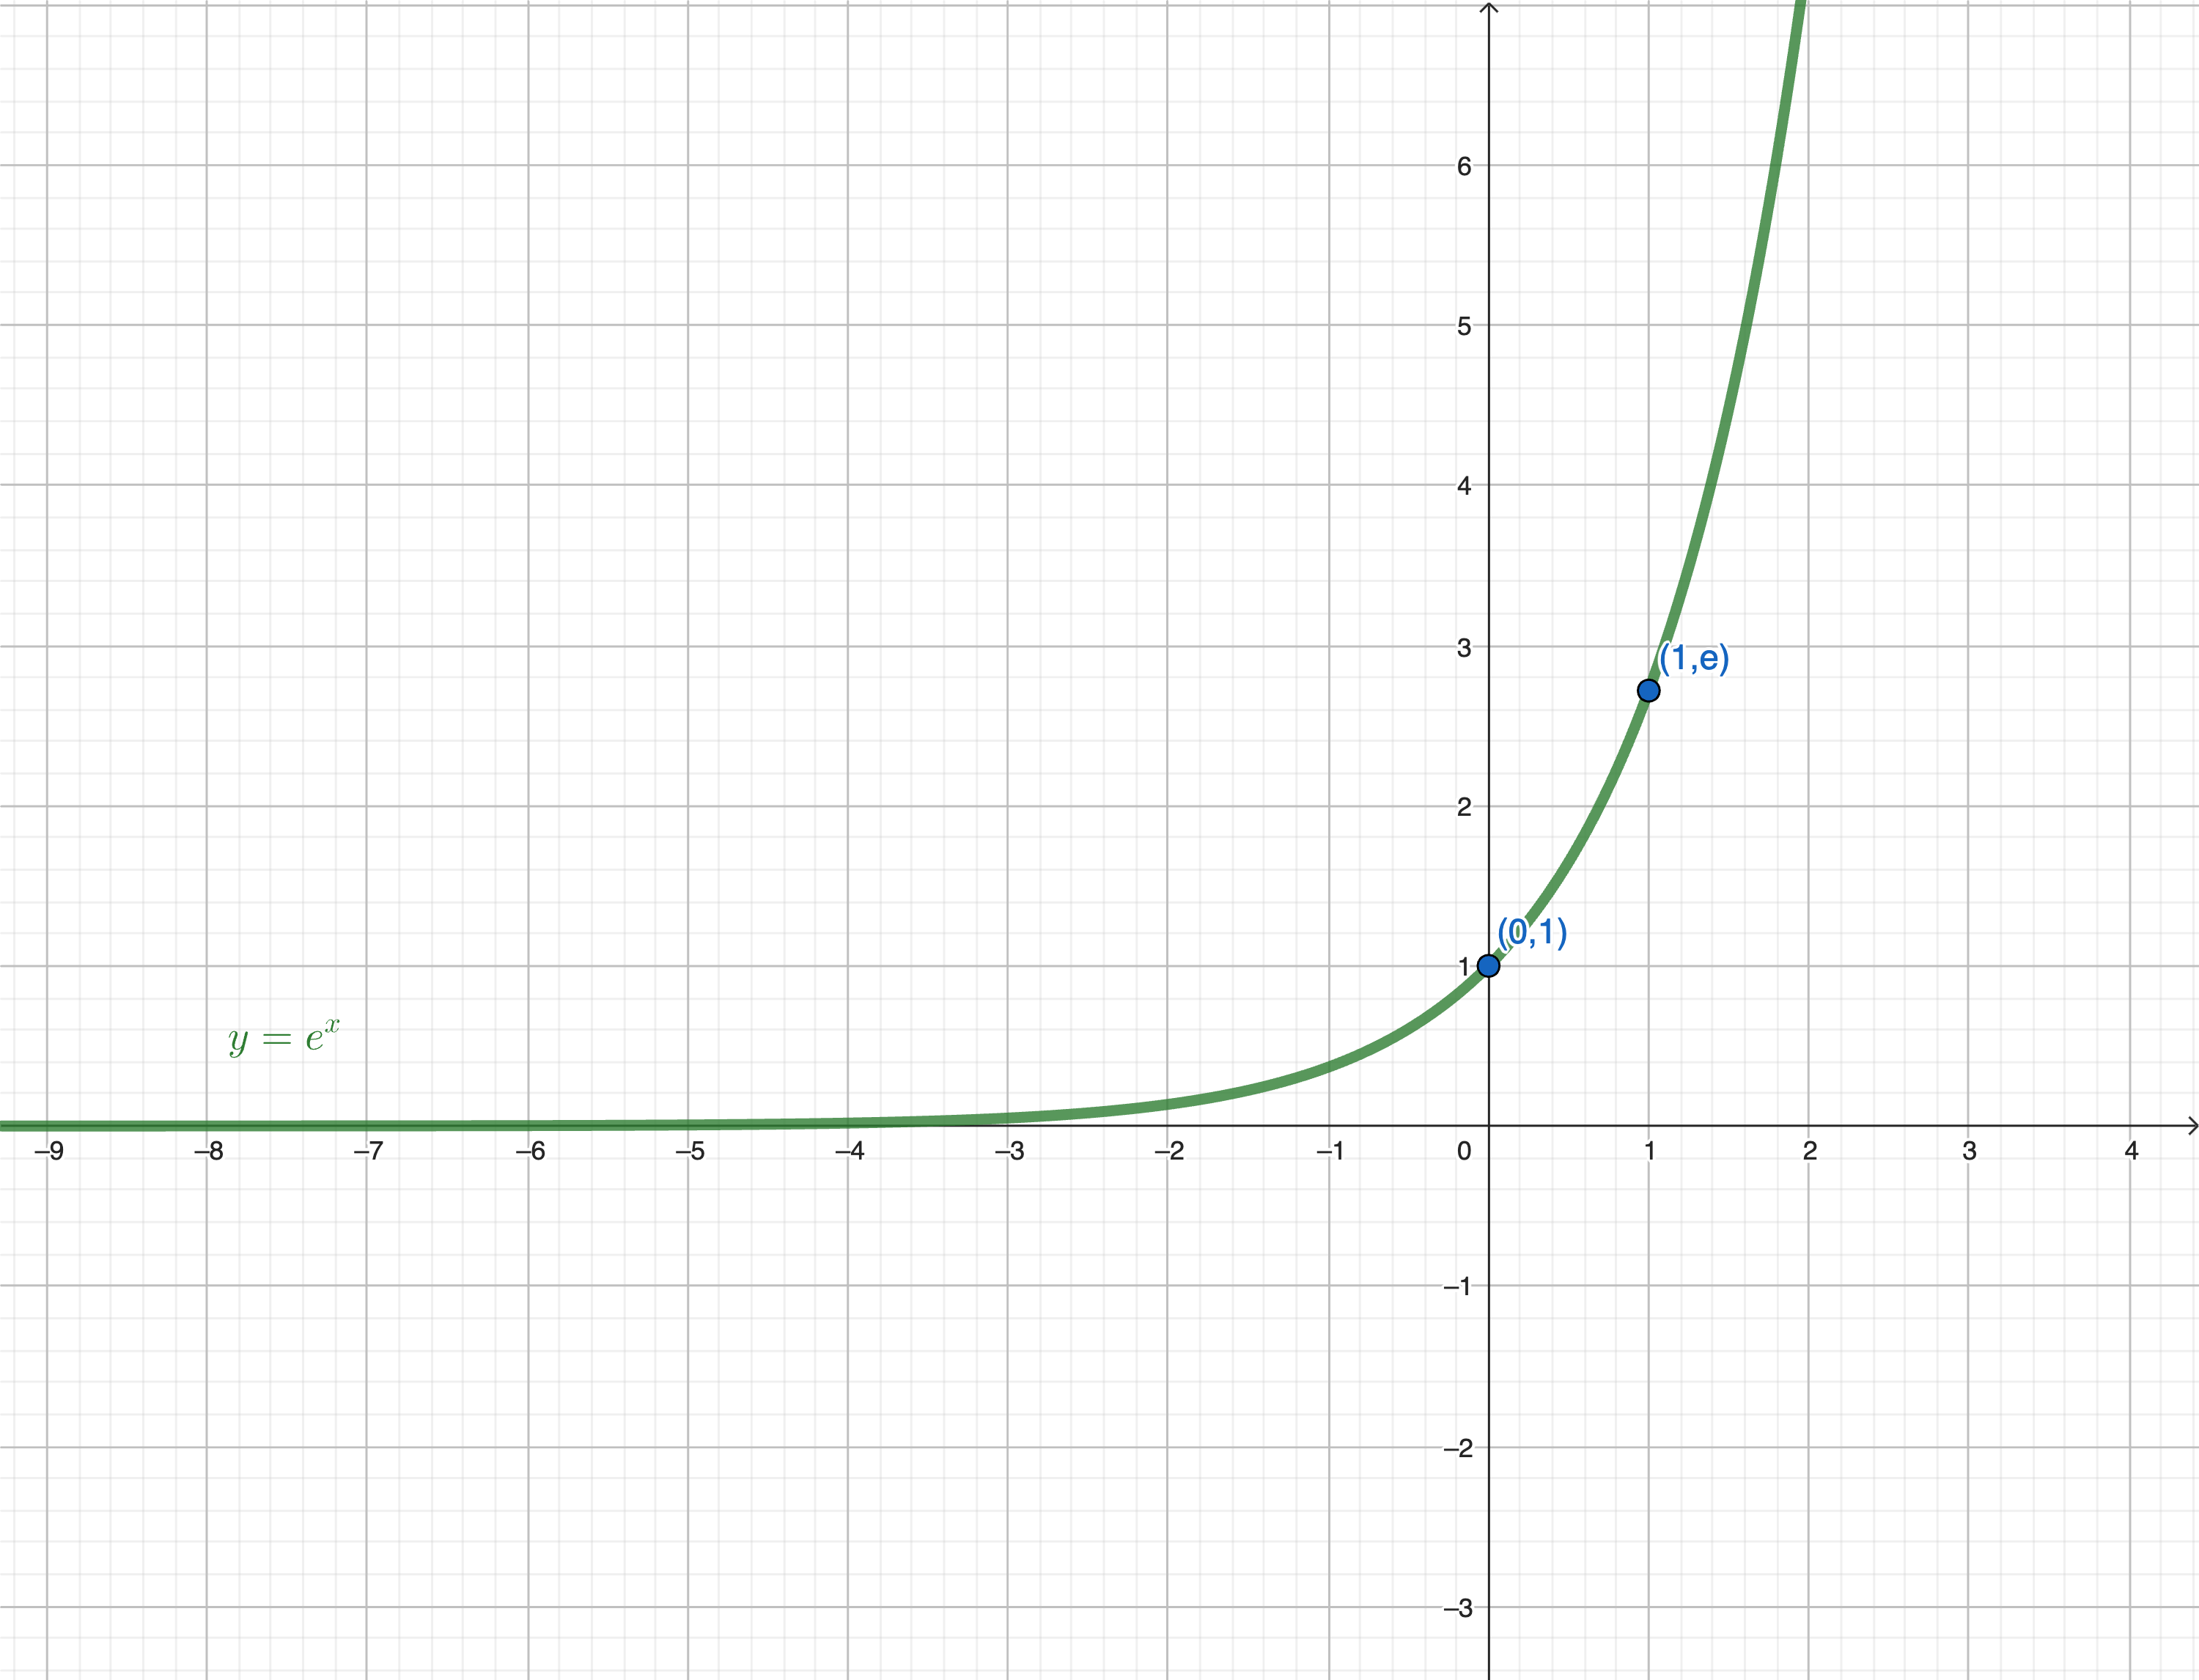
\includegraphics[width=.45\textwidth]{pics/exponencial.png}
\hfil
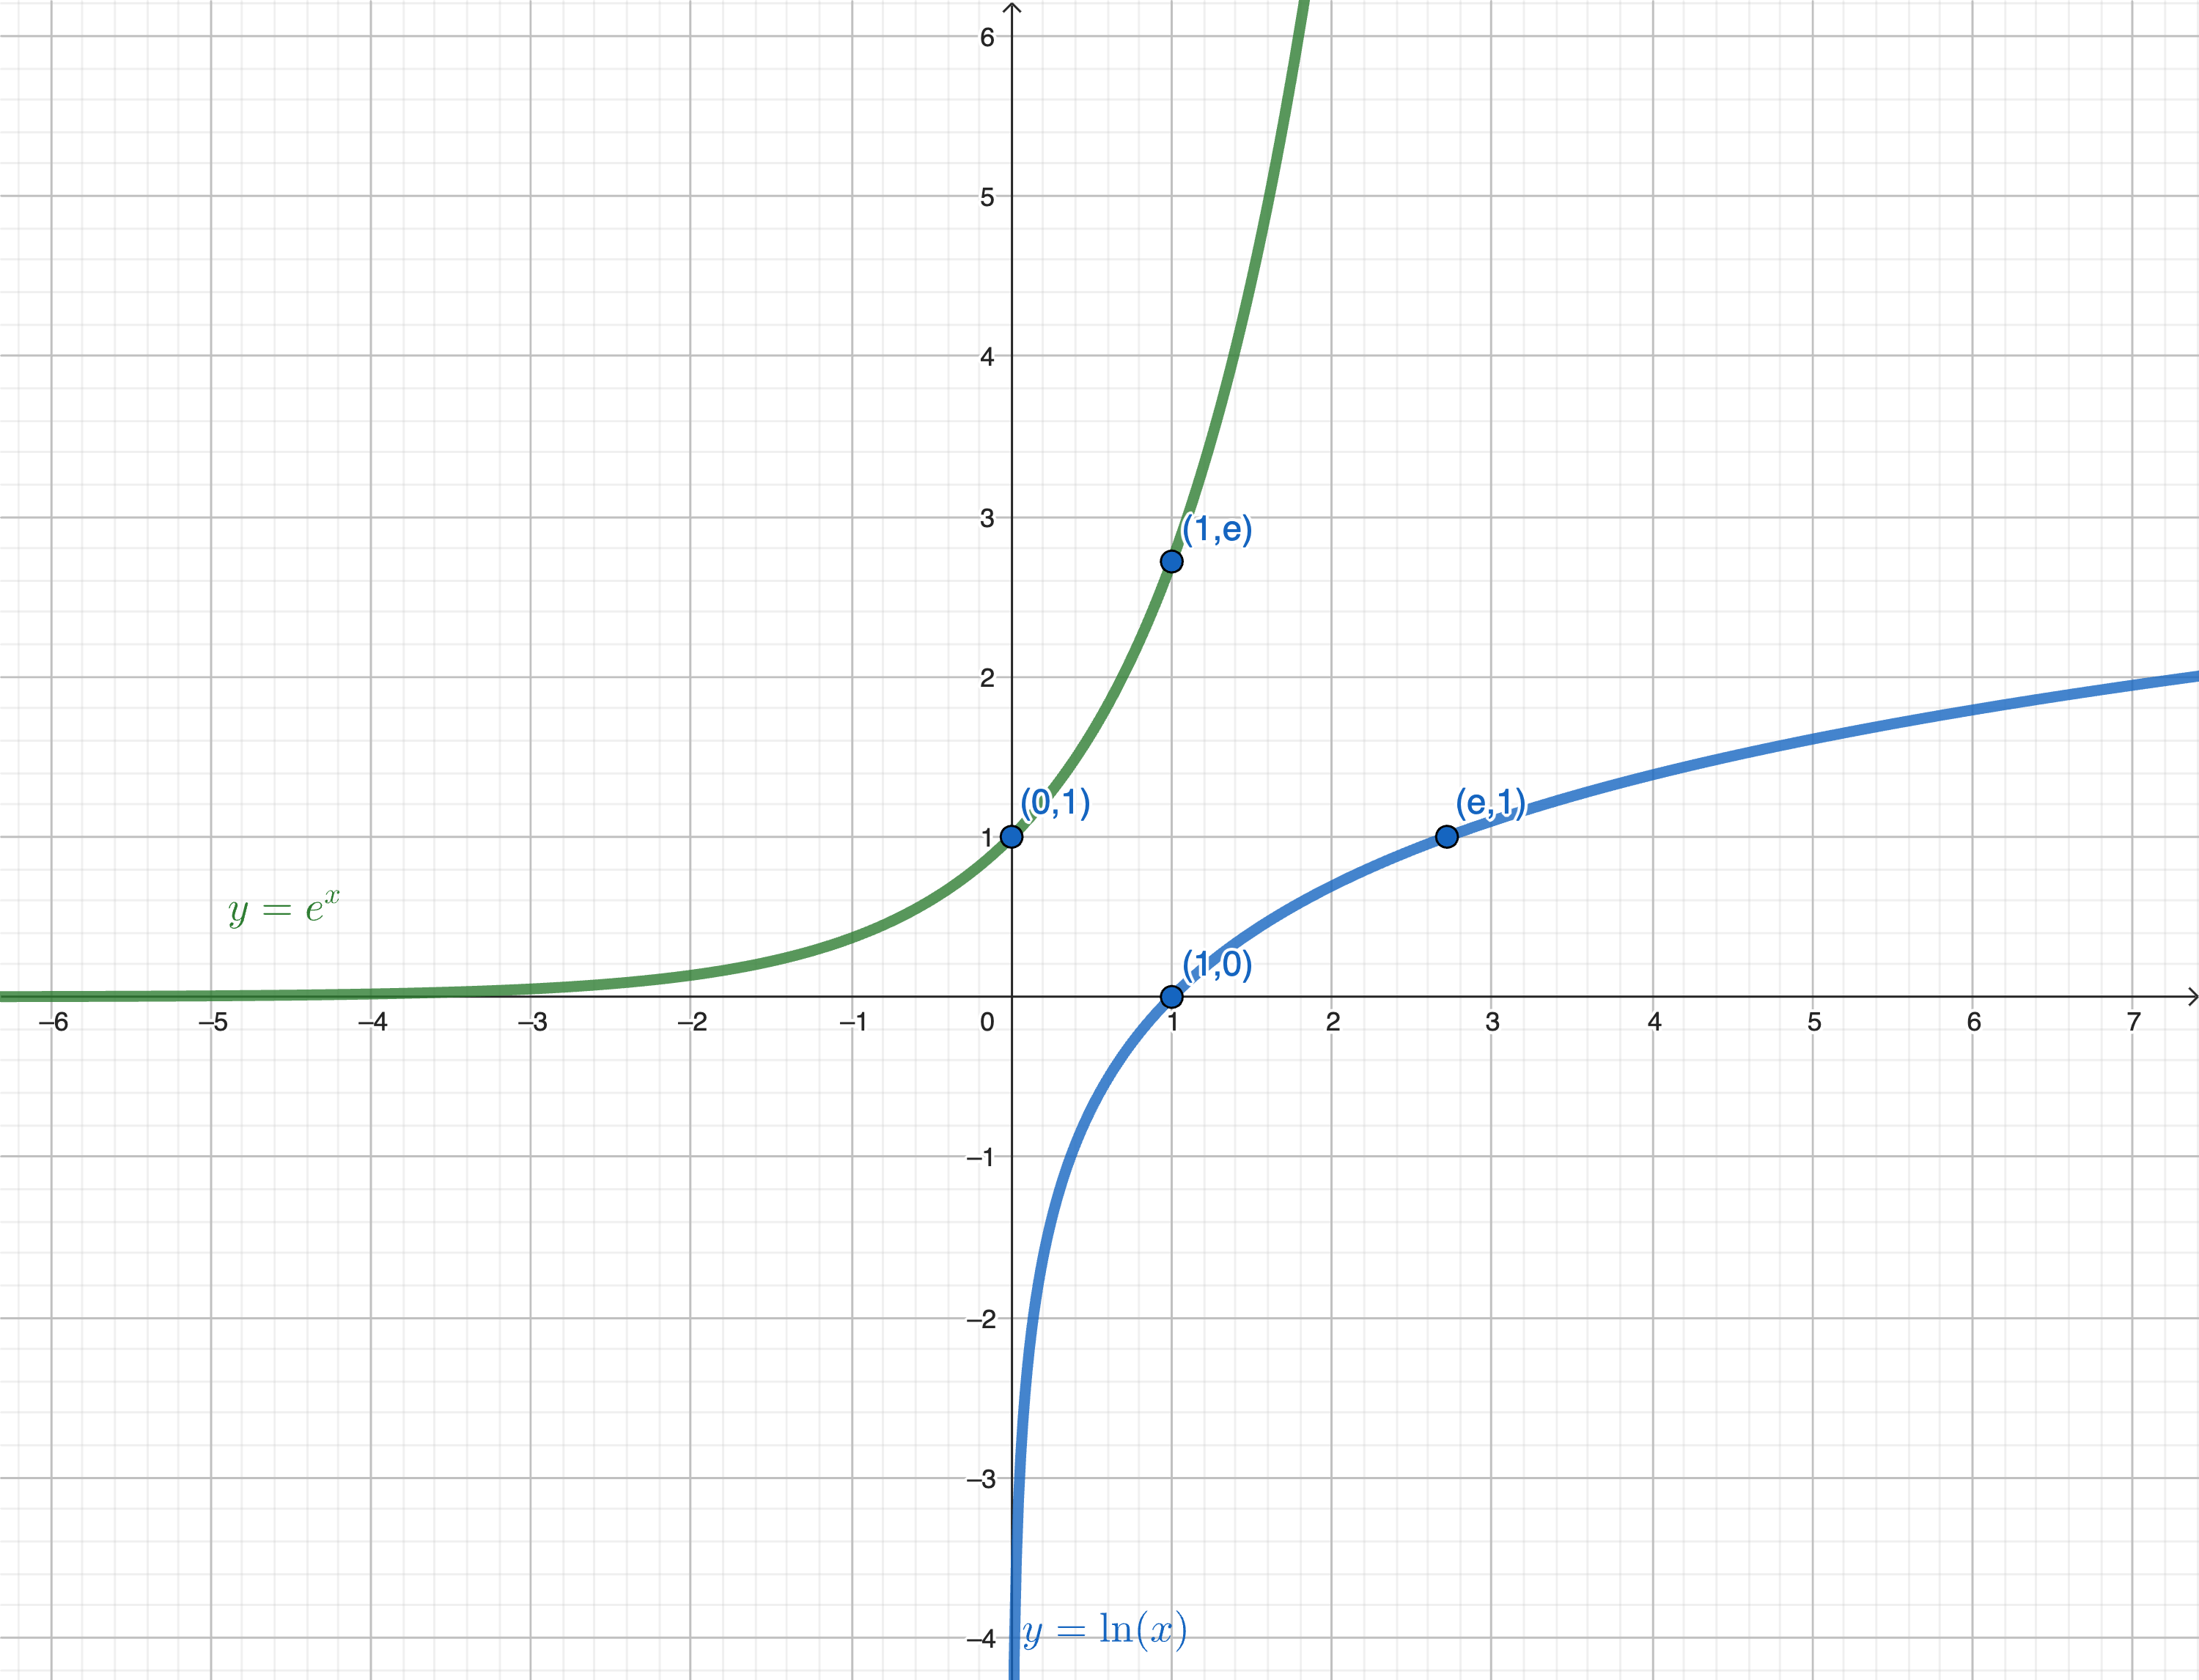
\includegraphics[width=.45\textwidth]{pics/exponencial-logaritmo.png}
}

Al ser $e^x$ biyectiva, tiene una función inversa, que es lo suficientemente importante como para recibir un nombre propio.

\begin{definition}
    Si $f:\R\to(0,+\infty)$ está dada por $f(x) = e^x$, entonces su función inversa se denomina \emph{función logaritmo} o \emph{función logaritmo natural} y se indica con $\ln : (0,+\infty) \to \R$. Para cada número $x > 0$ existe un único $y=\ln x\in\R$ que cumple:
    \[
    \ln x = y 
    \qquad\iff\qquad
    e^y = x.
    \]
    Dicho $y$ se llama \emph{logaritmo natural de $x$}.
\end{definition}

A partir de las propiedades enunciadas en el Teorema~\ref{T:exponencial propiedades} podemos deducir lo siguiente.

\begin{proposition}\label{P:logaritmo propiedades}
        \begin{enumerate}
        \item Si $x,y>0$, entonces $\ln (x\cdot y) = \ln(x) + \ln(y)$.
        \item Si $x > 0$ y $y\in\R$, entonces $\ln x^y = y \cdot \ln x$.
    \end{enumerate}
\end{proposition}

\begin{proof}
Ejercicio.
\end{proof}


De manera similar a como se hizo en el Teorema~\ref{P:exp biyectiva} se puede probar la siguiente proposición.

\begin{proposition}
    Si $a>0$, $a\neq 1$, la función $f:\R \to (0,+\infty)$ dada por $f(x) = a^x$ es biyectiva. Si $a>1$ $f$ es creciente y si $a<1$ $f$ es decreciente.
\end{proposition}

?`Por qué piensa el lector que no se estudia la función $a^x$ para $a=1$? ?`Y para $a<0$?

\begin{definition}
    Si $a>0$, $a\neq 1$, se define la función \emph{logaritmo en base $a$} como la inversa de $a^x$, es decir
    \[
    \log_a x = y \qquad\iff\qquad a^y = x.
    \]
    Es decir, el logaritmo en base $a$ de $x$ es la potencia a la que se debe elevar $a$ para obtener $x$.
\end{definition}

Para finalizar esta sección, demostramos la siguiente propiedad, realmente sorprendente.

\begin{proposition}
    Si $a>0$, entonces $\D \lim n (\sqrt[n]{a}-1) = \ln a$.
\end{proposition}

\begin{proof}
    Consideremos primero el caso $a\ge 1$ y sea $x=\ln a$, es decir, $e^x=a$, con $x\ge 0$.
    En primer lugar, recordemos que por el ejercicio~\ref{ej:eab} de la Sección~\ref{S:numero e}, tenemos que 
    \[
    \lim\big(1+\frac xn\big)^n = e^x.
    \]
    Veamos ahora que 
    \begin{align*}
        n (\sqrt[n]{a}-1) - \ln a &= n (\sqrt[n]{a}-1) - x 
        = n (\sqrt[n]{a}-1) - n\big( (1+\frac xn\big)^{n/n} - 1\big)
        \\
        &= n \left[ \sqrt[n]{a} - \sqrt[n]{(1+\frac xn\big)^n} \right].
    \end{align*}
    Esta última expresión es mayor o igual a cero, pues $(1+\frac xn)^{1/n}$ tiende \emph{crecientemente} a $e^x=a$.
    
    Si llamamos $\alpha = \sqrt[n]{a} $ y $\beta =  \sqrt[n]{(1+\frac xn\big)^n}$, tenemos que 
    \begin{align*}
    0\le \alpha - \beta 
    &= \frac{(\alpha-\beta)(\alpha^{n-1}+\alpha^{n-2}\beta + \dots +\alpha \beta^{n-2}+\beta^{n-1})}{\alpha^{n-1}+\alpha^{n-2}\beta + \dots +\alpha \beta^{n-2}+\beta^{n-1}}
    \\
    &= \frac{\alpha^n-\beta^n}{\alpha^{n-1}+\alpha^{n-2}\beta + \dots +\alpha \beta^{n-2}+\beta^{n-1}}.
    \end{align*}
    Como $x\ge 0$, $\beta \ge 1$, y como $a\ge 1$, también $\alpha \ge 1$.
    Por lo tanto, el denominador de la última expresión es mayor o igual a $n$, es decir, 
    \[
    \left[ \sqrt[n]{a} - \sqrt[n]{(1+\frac xn\big)^n} \right] 
    = \alpha - \beta \le \frac{\alpha^n - \beta^n) }n
    = \frac{ a - (1+\frac xn\big)^n}n
    \]
    Luego, 
    \[
    0\le n (\sqrt[n]{a}-1) - \ln a \le  a - (1+\frac xn\big)^n 
    = e^x - (1+\frac xn\big)^n\to 0, \quad\text{cuando $n\to\infty$}.
    \]
    Por el teorema del emparedado, $\lim n (\sqrt[n]{a}-1) - \ln a =0$, o lo que es lo mismo,
    $\lim n (\sqrt[n]{a}-1) = \ln a $.

    Si $0<a<1$, entonces $\ln a = - \ln \frac1a$ y $\frac1a>1$.
    Por lo que acabamos de ver
    \[ 
    \lim n \big(\sqrt[n]{\frac1a}-1\big) = \ln 1/a,
    \]
    pero 
    \[
    n \big(\sqrt[n]{\frac1a}-1\big) 
    = \frac{1}{\sqrt[n]{a}} n \big(1-\sqrt[n]{a}\big)
    = -\frac{1}{\sqrt[n]{a}} n \big(\sqrt[n]{a}-1\big).
    \]
    Esto implica que 
\[
n \big(\sqrt[n]{a}-1\big) = -\underbrace{\sqrt[n]{a}}_{\to 1} \underbrace{n \big(\sqrt[n]{\frac1a}-1\big) }_{\to \ln \frac1a} 
\to - 1 \cdot \ln\frac1a = \ln a.
\]
Hemos probado entonces el resultado que queríamos, tanto para $a\ge 1$ como para $0<a<1$. Es decir, para todo $a>0$.
    \end{proof}

\subsubsection*{Ejercicios de la sección~\getcurrentref{chapter}.\getcurrentref{section}}

\begin{enumerate}
\item Demostrar la Proposición~\ref{P:logaritmo propiedades}.

\item Demostrar las siguientes propiedades del logaritmo para $a>0$, $a\neq 1$:
\begin{enumerate}
    \item $\log_a (x\, y) = \log_a(x) + \log_a(y)$, para $x,y\in(0,+\infty)$.
    \item $\log_a (x^ y) = y \, \log_a(x)$, para $x\in(0,+\infty)$, $y\in\R$.
    \item $a^x = e^{x \ln a}$, para $x\in\R$.
    \item $\D\log_b x = \frac{\log_a(x)}{\log_a(b)}$, para $b>0$, $b\neq 1$ y $x>0$.
\end{enumerate}

\item Demostrar que $\log_a$ es creciente si $a>1$ y decreciente si $0<a<1$.

\item Sean $a,b > 0$. Probar que cualquiera sea $x \in \R$ se cumple que
\[
\text{a)}\quad (a\,b)^x = a^x\,b^x,
\qquad
\text{b)}\quad \Big(\frac ab\Big)^x = \frac{a^x}{b^x}.
\]
Ayuda: calcular $\ln(ab)^x$ y usar que $\ln$ es una función inyectiva.


\end{enumerate}


\section{Otras propiedades del límite}

Consideremos ahora una sucesión \sucan de términos positivos que tenga límite positivo $a$.
Podemos entonces considerar la sucesión que se obtiene tomando el logaritmo de cada término, es decir la sucesión $\big( \ln a_n \big)_\niN$ y también podemos considerar el logaritmo del límite $\ln a$. Lo que nos dice la siguiente proposición es que ambos resultados coinciden.

\begin{proposition}\label{P:logaritmo continuo}
    Sea \sucan una sucesión de términos positivos con límite también positivo:
    \[ 
    a = \lim a_n > 0.
    \]
    Entonces
    \[
    \lim \big(\ln a_n \big) = \ln a.
    \]
    O lo que es lo mismo
    \[
    \lim \big(\ln a_n \big) = \ln \big( \lim a_n \big).
    \]
\end{proposition}

\begin{proof}
    Sea $\epsilon>0$ arbitrario. Como $\lim a_n = a$ y $a\neq 0$, resulta $\lim \frac{a_n}a = 1$.
    Como $\epsilon>0$, $e^\epsilon > e^0=1$.
    Luego, existe $N_1\in\N$ tal que $\frac{a_n}{a} < e^\epsilon$, para todo $n\ge N_1$, y existe $N_2\in\N$ tal que $\frac{a_n}{a} > e^{-\epsilon}$, para todo $n\ge N_2$.
    Si definimos $N_0 = \max\{N_1,N_2\}$ entonces para $n\ge N_0$ se cumple que
    \[
    e^{-\epsilon} < \frac{a_n}a < e^\epsilon.
    \]
    Aplicando logaritmo, usando que el logaritmo es una función creciente, resulta
    \[
    \ln(e^{-\epsilon}) < \ln\big(\frac{a_n}a\big) < \ln(e^\epsilon),
    \qquad\text{para todo $n \ge N_0$},
    \]
    es decir,
    \[
    -\epsilon < \ln a_n - \ln a < \epsilon, \qquad\text{para todo $n \ge N_0$},
    \]
    que a su vez equivale a 
    \[
    |\ln a_n - \ln a| < \epsilon, \qquad\text{para todo $n \ge N_0$}.
    \]
    Hemos demostrado entonces que dado $\epsilon > 0$, existe $N_0\in\N$ tal que
    $|\ln a_n - \ln a| < \epsilon$, para todo $n \ge N_0$, o lo que es lo mismo, $\lim \ln a_n = \ln a$.
\end{proof}

La siguiente desigualdad será una herramienta útil en los resultados que siguen:

\begin{lemma}
    Sea $a > 1$. Entonces, para todo $x\in\R$ tenemos que
    \[
    \big| a^x - 1 \big| \le a^{|x|}-1.
    \]
\end{lemma}

\begin{proof}
Como $a>1$, la función $x\to a^x$ es creciente. Luego,
    si $x\ge 0$, se tiene que $a^x \ge a^0 = 1$ y por lo tanto
    \[
    \big| a^x - 1 \big| = a^x - 1 = a^{|x|} - 1,
    \]
    y la desigualdad deseada se cumple como igualdad.

    Veamos ahora qué ocurre cuando $x<0$. En este caso, $|x| = -x > 0$ y por lo tanto
    \begin{align*}
        \big| a^x - 1 \big| &= \big| 1 - a^x \big|
        = \big| 1 - \frac{1}{a^{-x}} \big|
        = \big| \frac{a^{-x} - 1}{a^{-x}} \big| 
        = \frac{1}{|a^{-x}|} |a^{-x}-1|
        \\
        &=  \frac{1}{a^{-x}} (a^{-x}-1)
        =  \frac{1}{a^{|x|}} (a^{|x|}-1)
        \le a^{|x|}-1.  \qedhere
    \end{align*}
\end{proof}

Ahora podemos demostrar que se puede tomar límite en una potencia:

\begin{lemma}\label{L:exp continua}
    Si $a>0$ y $\lim b_n = b$, entonces
    \[
    \lim a^{b_n} = a^b.
    \]
\end{lemma}

\begin{proof}
    La demostración de este lema hace uso del lema anterior. Supongamos primero que $a>1$. Luego
    \begin{align*}
        \big| a^{b_n} - a^b \big| 
        &= \big| a^{b_n-b+b} - a^b \big| 
        = \big| a^{b_n-b} a^b - a^b \big| 
        = \big| a^{b_n-b} - 1 \big| a^b
        \le \big( a^{|b_n-b|} - 1 \big) a^b.
    \end{align*}
    Sea ahora $k\in\N$ arbitrario. Como $\lim b_n = b$ existe $N_0\in\N$ tal que 
    \[
    |b_n-b|\le \frac1k,\qquad\text{para todo $n\ge N_0$}.
    \]
    Recordando la desigualdad de Bernoulli (Proposición~\ref{P:Bernoulli} con $h=a^{1/k}-1$ y $n=k$), tenemos que
    \[
    1 + k (a^{1/k}-1) \le \big(1 + (a^{1/k}-1)\big)^k = a,
    \]
    por lo que $\D a^{1/k}-1 \le \frac{a-1}k$.
    Luego
    \begin{align*}
        \big| a^{b_n} - a^b \big| 
        &\le \big( a^{|b_n-b|} - 1 \big) a^b
        \le  \big( a^{1/k} - 1 \big) a^b 
        \le \frac{a-1}k \, a^b.
    \end{align*}
    Sea ahora $\epsilon > 0$ y elijamos $k \in \N$ tal que 
    \[
    k > \frac{(a-1)\, a^b}{\epsilon}.
    \]
    Y sea $N_0\in\N$ que cumple lo anterior para ese $k$. Luego, para $n\ge N_0$ resulta
    \begin{align*}
        \big| a^{b_n} - a^b \big| 
        &< \frac{a-1}k \, a^b < \frac{a-1}{\frac{(a-1)\, a^b}{\epsilon}} \, a^b
        = \epsilon.
    \end{align*}    
    Hemos probado entonces que dado $\epsilon>0$, existe $N_0\in\N$ tal que
    \[
        \big| a^{b_n} - a^b \big| < \epsilon, \qquad\text{para todo $n\ge N_0$},
    \]
    es decir, $\lim a^{b_n} = a^b$. 

    Si $a=1$ el lema es trivial, pues $a^{b_n} = 1 = a^b$ para todo $n$.

    Si $0<a<1$, entonces $1/a>1$ y por lo que recién demostramos
    $\lim\big( 1/a \big)^{b_n} = 1/a$.
    Finalmente, por la Proposición~\ref{P:suc-lim-cociente}
    \[
    \lim a^{b_n} = \lim \frac{1}{(1/a)^{b_n}} = \frac{1}{\lim (1/a)^{b_n}}
     = \frac{1}{(1/a)^b} = a^b. \qedhere
    \] 
\end{proof}

La afirmación de este último lema era un caso particular de la siguiente proposición, pero un paso intermedio necesario para demostrarla.

\begin{proposition}\label{P:potencias continuas}
    Sea \sucan una sucesión de términos positivos con límite $a>0$ y sea \sucbn una sucesión con límite $b$. Entonces
    \[
    \lim a_n^{b^n} = a^b.
    \]
\end{proposition}

\begin{proof}
    Recordemos que el logaritmo natural es la función inversa de la función exponencial, así, para cualquier $x>0$, resulta $x = e^{\ln x}$. Aplicando esto a $x=a_n^{b_n}$ obtenemos
    \[
    a_n^{b^n} = e^{\ln a_n^{b_n }} = e^{b_n \ln a_n}.
    \]
    Si ahora consideramos la sucesión $c_n = b_n \ln a_n$, vemos que $\lim c_n = b \ln a$.
    Luego, por el lema anterior, $\lim e^{b_n \ln a_n} = e^{b \ln a} $, que finalmente implica lo siguiente:
    \[
    \lim a_n^{b^n} = \lim e^{b_n \ln a_n} = e^{b \ln a} = a^b. \qedhere
    \]
\end{proof}

Por último, también se cumplen las siguientes proposiciones, cuya demostración queda como ejercicio.

\begin{proposition}
    Si $a_n>0$ para todo \niN y $\lim a_n = 0$, entonces $\lim \ln(a_n) = -\infty$.
\end{proposition}
\begin{proof}
    Ejercicio.
\end{proof}

\begin{proposition}
    Si $\lim a_n = +\infty$, entonces $\lim \ln(a_n) = +\infty$.
\end{proposition}

\begin{proof}
    Ejercicio.
\end{proof}

\subsubsection*{Ejercicios de la sección~\getcurrentref{chapter}.\getcurrentref{section}}

\begin{enumerate}
\item Hallar los límites de las sucesiones dadas por:
\begin{multicols}{2}
    \begin{enumerate}
    \item $\D a_n = \Big( \frac{2n^2+3n-1}{3n^2-6n+1} \Big)^{2n}$
    \item $\D a_n = \Big( \frac{3n+4}{2n+5} \Big)^{\sqrt{n+1}-\sqrt{n}}$
    \item $\D a_n = \Big( \frac{3n+4}{3n-5} \Big)^{n}$
    \item $\D a_n = \Big( \frac{3n+4}{3n-5} \Big)^{n^2}$
    \item $\D a_n = \Big( \frac{3n+4}{3n-5} \Big)^{\sqrt{n}}$
    \item $\D a_n = \frac{\ln n}n$
    \end{enumerate}
\end{multicols}

\item Probar $\lim a_n = +\infty$ y $\lim b_n = b > 0$, entonces $\lim a_n^{b_n} = +\infty$.

\item Probar que si $\lim a_n = a > 1$ y $\lim b_n = +\infty$,
entonces $\lim a_n^{b_n} = +\infty$.

\end{enumerate}


\section{Teorema de Bolzano-Weierstrass}

En esta sección vamos a demostrar un teorema del cual haremos uso repetido en el resto del curso. Comenzamos con una definición.

\begin{definition}
    Un encaje de intervalos es una sucesión de intervalos cerrados $I_n = [a_n,b_n]$, con $a_n\le b_n$ tal que 
    \[
    I_1 \supset I_2 \supset I_3 \dots,
    \]
    es decir
    \[
    a_1 \le a_2 \le a_3 \le \dots,
    \qquad
    b_1 \ge b_2 \ge b_3 \ge \dots.
    \]
    En otras palabras, la sucesión \sucan es creciente y la sucesión \sucbn es decreciente, y además, todo $b_k$ es cota superior de \sucan y todo $a_k$ es cota inferior de \sucbn. Esquemáticamente:
    \[
    a_1 \le a_2 \le a_3 \le \dots
    \le b_3 \le b_2 \le b_1.
    \]
\end{definition}

Llamaremos \emph{longitud} del intervalo $I_n = [a_n,b_n]$ al número $b_n-a_n$, y lo denotaremos con $|I_n|$. Es decir, $|I_n| = |[a_n,b_n]| = b_n-a_n$.

\begin{theorem}
    Sea $(I_n)_\niN$ un encaje de intervalos que satisface $\lim |I_n| = 0$. Entonces existe un único $x \in \R$ que pertenece a todos los intervalos. Es decir
    \[
    \bigcap_{n=1}^\infty I_n = \{ x \}.
    \]
\end{theorem}

\begin{proof}
    Sean $a_n$, $b_n$ los extremos del intervalo $I_n$, es decir, $I_n=[a_n,b_n]$.
    Observemos que por la definición de encaje de intervalor, \sucan es creciente y acotada, por lo que existe $x=\lim a_n$. Ahora, como \sucan es creciente, $x \ge a_n$ para todo \niN.
    Por otro lado, $a_k \le b_n$, para todo $k,n\in\N$ , por lo tanto, $x 
    = \lim_{k\to\infty} a_k \le b_n$ para todo \niN. Es decir, $a_n\le x \le b_n$, o lo que es lo mismo, $x\in [a_n,b_n]=I_n$, para todo \niN.

    Ahora veamos la unicidad. Si $x,x' \in I_n$, para todo \niN, entonces 
    \[
    |x-x'| \le b_n-a_n = |I_n| \to 0,
    \]
    por lo que $|x-x'|=0$ o lo que es lo mismo, $x=x'$.
\end{proof}

Como consecuencia de este teorema se obtiene el \emph{Teorema de Bolzano-Weierstrass}, para lo cual tenemos que definir el concepto de \emph{subsucesión}, que consiste en elegir algunos elementos de una sucesión dada. Informalmente, una subsucesión de la sucesión \sucan es una sucesión de la forma:
    \[
    a_{n_1}, a_{n_2}, a_{n_3}, \dots,
    \]
    con $n_1<n_2<n_3<\dots$.

En otras palabras, si $\big(n_k\big)_{k\in\N}$ es una sucesión estrictamente creciente de números naturales, entonces $\big(a_{n_k}\big)_{k\in\N}$ es una subsucesión de \sucan.

Si recordamos que la definición de sucesión \sucan es como una función $a:\N\to\R$ donde denotamos $a_n = a(n)$, podemos definir precisamente una subsucesión de la siguiente manera.

\begin{definition}
Sea $a:\N\to\R$ una sucesión, e indiquemos $a_n=a(n)$. Una \emph{subsucesión} de \sucan es la composición
\[
a \circ n : \N \to \R
\]
de $a$ con una función \emph{estrictamente creciente} $n:\N \to \N$. Indicaremos $n_k = n(k)$ y luego $a_{n_k} = a_{n(k)} = a(n(k)) = a\circ n(k)$.
\end{definition}

Dos ejemplos claros de subsucesiones de una sucesión \sucan son los que se obtienen tomando los elementos de la sucesión que tienen índice par, o impar. Así, dos subsucesiones de \sucan son:
\[
a_2, a_4, a_6, \dots,\qquad\text{y}\qquad
a_1, a_3, a_5, \dots.
\]
La primera subsucesión es la que corresponde a $n_k = 2k$, $k\in\N$, que se denota $\big(a_{2k}\big)_{k\in\N}$ y la segunda es la que corresponde a $n_k = 2k-1$, $k\in\N$, que se escribe $\big(a_{2k-1}\big)_{k\in\N}$.

Hemos visto que toda sucesión convergente es acotada. 
La recíproca de esta afirmación no es cierta, ya que una sucesión acotada puede no ser convergente, por ejemplo la que está dada por $a_n = (-1)^n$.
Pero hay algo que se puede afirmar acerca de la convergencia de las sucesiones acotadas, y es lo que se plantea en el siguiente Teorema.

\begin{theorem}[Teorema de Bolzano-Weierstrass]
\label{T:Bolzano-Weierstrass} 
    Toda sucesión acotada contiene una subsucesión convergente.
\end{theorem}

\begin{proof}
    La demostración de este teorema es interesante y constructiva, y se verá en las clases de Coloquio de demostraciones.
\end{proof}

\subsubsection*{Ejercicios de la sección~\getcurrentref{chapter}.\getcurrentref{section}}

\begin{enumerate}
\item Consideremos las sucesiones
\[
b_n = \frac{1^2+2^2 + \dots + (n-1)^2}{n^3},
\qquad
c_n = \frac{1^2+2^2 + \dots + n^2}{n^3},
\]
e $I_n = [b_n,c_n]$.  Probar que $\big( I_n \big)_\niN$ es un encaje de intervalos cuyas longitudes tienden a cero. Hallar la intersección de todos ellos.

\item \begin{enumerate}
    \item 
Dar un ejemplo de un encaje de intervalos tal que la intersección de todos ellos contenga más de un punto.
\item* Probar que la intersección de todos los intervalos cerrados de un encaje de intervalos $\left(I_n\right)_{\niN}$ cualquiera es un intervalo cerrado. Ayuda: llamar $a_n$ y $b_n$ a los extremos izquierdo y derecho de $I_n$, respectivamente y luego definir $a = \sup \{a_n:\niN\}$ y $b = \inf\{b_n:\niN\}$; finalmente probar que la intersección es $[a,b]$.

\item Dar un ejemplo de una sucesión $\left(I_n\right)_{\niN}$ de intervalos \emph{abiertos} tales que $I_{n+1}\subset I_n$, $\forall\niN$ y tal que $\bigcap_{n=1}^\infty = \emptyset.$
\end{enumerate}

\end{enumerate}


\section{Sucesiones de Cauchy}

Antes, antes de entrar en tema, probamos un resultado sobre sucesiones y subsucesiones.

\begin{proposition}\label{P:caracterizacionporsubsucesiones}
    Una sucesión \sucan es convergente con límite $a$ si y sólo si toda subsucesión de \sucan es convergente con el mismo límite $a$.
\end{proposition}

\begin{proof}
Supongamos primero que $\lim a_n = a$ y sea \subsucan una subsucesión de \sucan. Es decir, $\left(n_k\right)_{k\in\N}$ es una sucesión estrictamente creciente de números naturales.
Dado $\epsilon > 0$, existe $N_0\in\N$ tal que 
\[
|a_n - a| < \epsilon, \quad\text{para todo $n\ge N_0$}.
\]
Ahora bien, como $n_k$ es una sucesión estrictamente creciente de números naturales, resulta que $n_k \ge k$, para todo $k\in\N$. Luego, si $k \ge N_0$, resulta que $n_k \ge k \ge N_0$ y luego $\big|a_{n_k} - a \big| < \epsilon$. Hemos probado que dado $\epsilon>0$ existe $N_0\in\N$ tal que 
\[
|a_{n_k} - a| < \epsilon, \quad\text{para todo $k\ge N_0$}.
\]
Es decir, $\lim_{k\to\infty} a_{n_k} = a$.

Supongamos ahora que toda subsucesión de \sucan converge con límite $a$. Entonces consideramos la subsucesión correspondiente a $n_k = k$, $k\in\N$, que coincide con la sucesión original.
Luego, esta subsucesión tiene límite $a$ y por lo tanto la sucesión original tiene límite $a$.
\end{proof}

Esta proposición es muy útil para demostrar cuando una sucesión no converge.
Si consideramos la sucesión \sucan dada por $a_n = (-1)^n$, vemos que la subsucesión $a_{2n}$ es la sucesión constantemente 1, que tiende a 1, y la subsucesión $a_{2n-1}$ es constantemente $-1$. Por lo tanto hay dos subsucesiones con diferente límite, y la sucesión original no converge.

Para definir sucesión convergente, lo que hicimos fue escribir de manera precisa la idea de que los términos de la sucesión se vayan acercando a un cierto número. Ahora, escribiremos de manera precisa la idea siguiente: que los términos de la sucesión se vayan acercando entre sí. Lo haremos de la siguiente manera:

\begin{definition}
    Se dice que una sucesión \emph{es de Cauchy} si cumple la siguiente propiedad:
    \begin{quote}
        Dado $\epsilon > 0$, existe $N_0 \in\N$ tal que
        \[
        \text{si $n,m\in\N$, $n\ge N_0$, $m\ge N_0$} \quad\text{entonces}\quad
        \big| a_n - a_m \big| < \epsilon.
        \]
    \end{quote}
\end{definition}

Veremos a continuación que una sucesión converge, sí, solo si es de Cauchy.
Comenzamos probando que toda sucesión de Cauchy es acotada.

\begin{proposition}\label{P:Cauchy=>Acotada}
    Si \sucan es una sucesión de Cauchy, entonces es acotada.
\end{proposition}

\begin{proof}
    Sea \sucan una sucesión de Cauchy. Consideremos $\epsilon = 1$ en la definición de sucesión de Cauchy. Luego, existe $N_0$ tal que, si $n,m\ge N_0$, resulta $|a_n-a_m|<1.$
    En particular, $|a_n - a_{N_0}| < 1$, para todo $n\ge N_0$. Es decir
    \[
    -a_{N_0} + 1 < a_n < a_{N_0} + 1, \qquad \text{para todo $n\ge N_0$}. 
    \]
    De esta manera, vemos que está acotada la sucesión a partir de $N_0$. Lo que resta es acotar los primeros $N_0$ términos, pero son un número finito de términos.
    Más precisamente, consideramos
    \begin{align*}
        M &= \max\{a_1, a_2, \dots, a_{N_0-1}, a_{N_0}+1\}, 
        \\
        m &= \min\{a_1, a_2, \dots, a_{N_0-1}, -a_{N_0}+1\}, 
    \end{align*}
    y entonces resulta que
    \[
    m \le a_n \le M, \qquad \text{para todo \niN}.
    \]
    Por lo tanto, la sucesión es acotada.
\end{proof}

El segundo paso de la demostración consiste en probar que si una sucesión de Cauchy tiene una subsucesión convergente, entonces toda la sucesión converge.

\begin{proposition}\label{P:Cauchy+subsuc=>convergencia}
    Sea \sucan una sucesión de Cauchy, y supongamos que existe una subsucesión \subsucan tal que $\lim_{k\to\infty} a_{n_k} = a$.
    \mara{Entonces la sucesión converge a $a$.}
\end{proposition}

\begin{proof}
    Sea $\epsilon>0$, arbitrario. Como la sucesión \sucan es de Cauchy, existe $N_0\in\N$ tal que
    \[
    |a_n - a_n | < \frac\epsilon2,\qquad\text{para todo $n,m\ge N_0$}.
    \]
    Como la subsucesión \subsucan converge a $a$, existe $N_0'\in\N$ tal que 
    \[
    | a_{n_k} - a | < \frac\epsilon2,\qquad\text{para todo $k \ge N_0'$}.
    \]
    En particular, si $k_0 \ge \max\{N_0,N_0'\}$, $n_{k_0} \ge k_0 \ge \max\{N_0,N_0'\}$ y resulta, para $n\ge N_0$,
    \[
    |a_n - a| = |a_n - a_{n_{k_0}} + a_{n_{k_0}} - a|
    \le |a_n - a_{n_{k_0}}| + |a_{n_{k_0}} - a|
    < \frac\epsilon2 + \frac\epsilon2 = \epsilon,
    \]
    lo cual prueba la afirmación de la proposición.
\end{proof}

Ahora estamos en condiciones de probar el resultado anunciado.

\begin{theorem}\label{T:converge sii Cauchy}
    Una sucesión es convergente si y sólo si es de Cauchy.
\end{theorem}

\begin{proof}
    Supongamos primero que \sucan es convergente con límite $a$. Entonces, dado $\epsilon>0$ existe $N_0\in\N$ tal que, si $n\ge N_0$, resulta $|a_n-a|<\epsilon/2$.
    Luego, si $n,m\ge N_0$,
    \[
    |a_n - a_m| = |a_n - a + a - a_m| \le |a_n-a| + |a-a_m| 
    < \frac\epsilon2 + \frac\epsilon2 = \epsilon.
    \]
    Hemos demostrado entonces que la sucesión es de Cauchy.

    Supongamos ahora que la sucesión es de Cauchy. Entonces, por la Proposición~\ref{P:Cauchy=>Acotada} la sucesión resulta acotada y por el Teorema~\ref{T:Bolzano-Weierstrass} debe contener una subsucesión convergente.
    Finalmente, la Proposición~\ref{P:Cauchy+subsuc=>convergencia}, la sucesión resulta convergente.
\end{proof}

\subsubsection*{Ejercicios de la sección~\getcurrentref{chapter}.\getcurrentref{section}}

\begin{enumerate}
\item Demostrar que si $\left(n_k\right)_{k\in\N}$ es una sucesión estrictamente creciente de números naturales, entonces $n_k \ge k$, para todo $k\in\N$.
\item * Probar que una sucesión es de Cauchy si y sólo si dado $\epsilon>0$ existe $N_0\in\N$ tal que, para $n\ge N_0$ se cumple que
\[
|a_{n+p} - a_n| < \epsilon,\quad \text{cualquiera sea $p\in\N$}.
\]

\item Probar que si una sucesión es de Cauchy, entonces, cualquiera sea $p\in\N$ se cumple que
$\D\lim_{n\to\infty} (a_{n+p}-a_n) = 0$.

\item Mostrar que la recíproca del ejercicio anterior no es cierta. Ayuda. Considerar la sucesión dada por $a_n = \ln n$, ?`Cuál es $\lim a_n$? ?`Cuál es $\D\lim_{n\to\infty} (a_{n+p}-a_n)$? 

\item Demostrar que la sucesión dada por $a_n = (-1)^n+\frac1n$ no es convergente.

\item Encontrar tres ejemplos de sucesiones acotadas que no sean convergentes.


\end{enumerate}

\section{Ejercicios del capítulo~\getcurrentref{chapter}}
\begin{enumerate}
\input{ejercicios-ch-2-s-01}
\item Probar que la sucesión \emph{constante} $a_n=a$ para todo $n\in\N$, tiene límite $a$.

\item Probar que si $\lim a_n = a$, entonces $\lim |a_n| = |a|$ (ayuda, usar la desigualdad triangular del ejercicio~\ref{ej:triangular resta} del Capítulo~\ref{Cap:Reales}).

\item Probar las siguientes afirmaciones:

\begin{multicols}{2}
    \begin{enumerate}
        \item $\D \lim \frac1{\sqrt{n}} = 0 $
        \item $\D \lim \frac{1}{\sqrt{n+1}+\sqrt{n}} = 0 $
        \item $\D \lim \frac{(-1)^n}{3n^2-4n} = 0 $
        \item $\D \lim \frac{(-1)^{n-1}}{2-n^2} = 0 $
        \item $\D \lim \frac{n}{n+1} = 1 $
        \item $\D \lim \frac{3n}{4n+2} = \frac34 $
        \item $\D \lim \frac{2n+3}{n^2-2n-3} = 0 $
        \item $\D \lim \frac{-3n+1}{4n^2-3n+4} = 0 $
        \item $\D \lim \frac{3n^2+2n-2}{n^2+1} = 3 $
        \item $\D \lim \frac{2n^2-3n+1}{3n^2+2n-1} = \frac23 $
        \item $\D \lim \frac{n^2+n+1000}{3n^2-14n-7} = \frac13 $
        % \item $\D \lim \frac{n}{n^{3/2}+1} = 0 $
        % \item $\D \lim \frac{n^{2/3}+100}{n^{3/4}+4} = 0 $
        % \item $\D \lim \frac{3n^{2/3}+n^{4/5}+2n^{5/2}}{n^3+n^{2/3}+5n} = 0 $
        % \item $\D \lim \frac{2n^{3/4}+\sqrt n}{n^{3/4}} = 2 $
        % \item $\D \lim \frac{n^2-3n^{7/2}+20}{n^{7/2}-6n^3+3n^2-2n} = -3$
    \end{enumerate}
\end{multicols}

\item Probar que $\D \lim \big( \sqrt{n+1} - \sqrt{n}\big) = 0$.
(Sugerencia: multiplicar y dividir por \emph{el conjugado} $\sqrt{n+1} + \sqrt{n}$)

\item Sea $\big( a_n \big)_{n\in\N}$ una sucesión convergente con límite $\ell$. Probar que si $\big(b_n \big)_{n\in\N}$ está definida por 
\[
b_n = a_{n+1}, \qquad \text{o sea $b_1=a_2$, $b_2=a_3$, $b_3=a_4$, \dots},
\]
entonces $\D\lim b_n = \ell$.

\item Sea $\big( a_n \big)_{n\in\N}$ una sucesión convergente con límite $\ell$, y sea $p\in\N$.
Probar que si $\big(b_n \big)_{n\in\N}$ está definida por 
\[
b_n = a_{n+p}, \qquad \text{o sea $b_1=a_{p+1}$, $b_2=a_{p+2}$, $b_3=a_{p+3}$, \dots},
\]
entonces $\D\lim b_n = \ell$.

\item Sea $\big( a_n \big)_{n\in\N}$ una sucesión convergente con límite $\ell$, y sea $p\in\N$.
Probar que si $\big(b_n \big)_{n\in\N}$ está definida por 
\[
\begin{cases}
    b_1 &= \text{cualquier cosa},\\
b_2 &= \text{cualquier cosa},\\
 &\vdots\\
b_p &= \text{cualquier cosa},
\end{cases}
\qquad\qquad \text{y }\quad b_k = a_k, \ \text{ para } \ k>p,
\]
entonces $\D\lim b_n = \ell$.

\item Probar que si \sucan es una sucesión convergente y $c$ es un número real cualquiera, entonces $\lim (c \, a_n) = c\, \lim a_n$.

\item Probar que si \sucan es convergente y $k$ es un número \emph{natural} cualquiera, entonces $\lim a_n^k = \left(\lim a_n\right)^k$. (Ayuda: razonar por inducción sobre $k$ y usar la Proposición~\ref{P:suc-lim-prod})

\item Determinar cuáles de las siguientes afirmaciones son verdaderas y cuáles no (en caso afirmativo, dar una demostración, en caso negativo, un contraejemplo).
\begin{enumerate}
    \item Si $(a_n+b_n)_\niN$ es convergente, entonces \sucan y \sucbn son convergentes.
    \item Si $(a_n+b_n)_\niN$ es convergente y $\sucan$ es convergente, entonces \sucbn es convergente.
    \item Si $(a_n\cdot b_n)_\niN$ es convergente, entonces \sucan y \sucbn son convergentes.
    \item Si $(a_n\cdot b_n)_\niN$ es convergente y \sucan es convergente, entonces \sucbn es convergente.
    \item Si $(a_n\cdot b_n)_\niN$ es convergente y \sucan es convergente con límite distinto de cero, entonces \sucbn es convergente.
    \item Si $(a_n^2)_\niN$ es convergente, entonces \sucan es convergente.
    \item Si \sucan es convergente con límite cero y \sucbn es acotada, entonces $(a_n\cdot b_n)_\niN$ es convergente con límite cero.
\end{enumerate}

\item Calcular los siguientes límites:

\begin{multicols}{2}
    \begin{enumerate}
        \item $\D \lim \frac{3n^3+4n^2-6}{7+8n+9n^3} $
        \item $\D \lim \frac{1-2n+3n^2}{4+5n-6n^2} $
        \item $\D \lim \frac{1-2n+3n^2}{4+5n-6n^2+n^3} $
        \item $\D \lim \frac{1}{2 n^{3/2}} $
        \item $\D \lim \frac{1000 + 10 n - 2 n^{3/2}}{10 n^{3/2}} $
        \item $\D \lim \frac{1000 + 10 n - 2 n^{3/2}}{10 n^{3/2}-n^2} $

        \item $\D \lim \frac{n}{n^{3/2}+1} = 0 $
        \item $\D \lim \frac{n^{2/3}+100}{n^{3/4}+4} = 0 $
        \item $\D \lim \frac{3n^{2/3}+n^{4/5}+2n^{5/2}}{n^3+n^{2/3}+5n} = 0 $
        \item $\D \lim \frac{2n^{3/4}+\sqrt n}{n^{3/4}} = 2 $
        \item $\D \lim \frac{n^2-3n^{7/2}+20}{n^{7/2}-6n^3+3n^2-2n} = -3$
\end{enumerate}
\end{multicols}


    \item Calcular los siguientes límites:

    \begin{multicols}{2}
        \begin{enumerate}
            \item $\D \lim \frac{3n^4+4n^2-6}{7+8n+9n^3} $
            \item $\D \lim \frac{1-2n+3n^3}{4+5n-6n^2} $
            \item $\D \lim \frac{1-2n+3n^2}{4+5n-6n^2+n^3} $
            \item $\D \lim \frac{n^{3/2}}{10n+1} $
            \item $\D \lim \frac{1000 + 10 n - 2 n^{5/2}}{10 n^{3/2}} $
            \item $\D \lim \frac{1000 + 10 n - 2 n^{3/2}+n^2}{10 n^{3/2}-n^2} $
        \end{enumerate}
    \end{multicols}
    
\item Demostrar que si $r>0$ y \sucan es una sucesión tal que $|a_n| > r$, para todo \niN y \sucbn es una sucesión tal que $b_n\neq 0$ para todo $n$ y $\lim b_n = 0$, entonces
\[ \lim \frac{a_n}{b_n} = \infty. \]
Esto daría la regla de cálculo $\D\frac{a}{0} = \infty$ si $a\neq 0$.

\item Probar las siguientes afirmaciones
\begin{enumerate}
    \item Si \sucan es acotada y $\lim b_n = +\infty$, entonces $\lim\big(a_n+b_n) = +\infty$.
    \item Si \sucan es acotada y $\lim b_n = -\infty$, entonces $\lim\big(a_n+b_n) = -\infty$.
    \item Si $\lim a_n = +\infty$ y $\lim b_n = +\infty$, entonces $\lim\big(a_n+b_n) = +\infty$.
    \item Si $\lim a_n = -\infty$ y $\lim b_n = -\infty$, entonces $\lim\big(a_n+b_n) = -\infty$.
    \item Si $\lim a_n = +\infty$ y $\lim b_n = -\infty$, entonces $\lim\big(a_n\cdot b_n) = -\infty$.
\end{enumerate}

\item Mostrar, dando un contraejemplo en cada caso, que las siguientes afirmaciones son falsas.
\begin{enumerate}
    \item Si $\lim a_n = \infty$ y $\lim b_n = \infty$, entonces $\lim\big(a_n + b_n) = \infty$.
    \item Si $\lim a_n = a$ y $\lim b_n = \infty$, entonces $\lim\big(a_n \cdot b_n) = \infty$.
\end{enumerate}

\item Probar las siguientes afirmaciones:
\begin{enumerate}
    \item Si $\lim b_n = +\infty$ y $a_n \ge b_n$ para todo \niN, entonces $\lim a_n = +\infty$.
    \item Si $\lim b_n = -\infty$ y $a_n \le b_n$ para todo \niN, entonces $\lim a_n = -\infty$.
    \item Si $\lim a_n = a > 0$ y $\lim b_n = +\infty$, entonces $\lim\big(a_n\cdot b_n\big) = +\infty$.
    \item Si $\lim a_n = a < 0$ y $\lim b_n = +\infty$, entonces $\lim\big(a_n\cdot b_n\big) = -\infty$.
\end{enumerate}

\item Sean $f$ y $g$ funciones polinómicas de grados $h$ y $k$ respectivamente. Para cada natural $n$ están definidos $f(n)$ y $g(n)$. Probar
\[
\textbf{(a)}\quad \lim\frac{f(n)}{g(n)} = 0, \ \text{si $h<k$},
\qquad
\textbf{(b)}\quad \lim\frac{f(n)}{g(n)} = \infty, \ \text{si $h>k$}.
\]
?`Cuánto vale $\D \lim\frac{f(n)}{g(n)}$ si $h=k$?



\item Sea \sucan una sucesión tal que se cumple lo siguiente:
\begin{quote}
Existen $r,R$ positivos tales que $r < a_n < R$, para todo $n\in\N$.
\end{quote}
Demostrar que entonces $\lim \sqrt[n]{a_n} = 1$. 

\item Sea \sucan una sucesión convergente de términos positivos tal que:
\[
\lim a_n > 0.
\]
Demostrar que entonces $\lim \sqrt[n]{a_n} = 1$. 

\item Dar un ejemplo de una sucesión \sucan acotada y de términos positivos para la cual no sea cierto que $\lim \sqrt[n]{a_n} = 1$. 

\item Probar las siguientes afirmaciones.
\begin{enumerate}
    \item $\lim  \sqrt[n]{n^2} = 1$.
    \item $\lim  \sqrt[n]{n^3} = 1$.
    \item Si $k\in\N$, entonces $\lim \sqrt[n]{n^k} = 1$.
\end{enumerate}

\item Probar las siguientes afirmaciones.
\begin{enumerate}
    \item $\lim \sqrt[n]{n^2+n} = 1$.
    \item $\lim \sqrt[n]{n^2-n} = 1$.
    \item $\lim \sqrt[n]{3n^3+2n^2+2n+1} = 1$.
    \item $\lim \sqrt[n]{3n^3-4n^2+6n-3} = 1$.
\end{enumerate}

\item Calcular
\begin{enumerate}
    \item $\lim \sqrt[n]{3^n+2}$
    \item $\lim \sqrt[n]{3^n-2}$
    \item $\lim \sqrt[n]{(\frac12)^n+3}$
    \item $\lim \sqrt[n]{3^n+2^n}$
    \item $\lim \sqrt[n]{a^n+b^n}$, si $0 < a < b$.
\end{enumerate}

\item Sea \sucan una sucesión convergente con límite $a$.
Probar que
\begin{enumerate}
    \item $\lim a_n^n = +\infty$, si $a>1$.
    \item $\lim a_n^n = \infty$, si $a<-1$.
    \item $\lim a_n^n = 0$, si $|a|<1$.
\end{enumerate}
    \item Para las siguientes sucesiones, decir cuáles son crecientes, cuáles estrictamente crecientes, cuáles decrecientes, cuáles estrictamente decrecientes, y cuáles acotadas:
    \begin{multicols}{2}
        \begin{enumerate}
        \item $\D a_n = \frac{n}{n+1}$
        \mara{\item $\D b_n = \frac{n^2}{n+1}$}
        \item $\D c_n = \frac{n!}{n^n}$
        \item $\D d_n = \frac{1}{\sqrt{n+1}-\sqrt{n}}$
        \item $\D e_n = \frac{1}{n+1} + \frac{1}{n+2} + \dots + \frac{1}{2n}$
        \mara{\item $\D f_n = \frac{2^n-1}{2^n} $}
    \end{enumerate}
    \end{multicols}
\item Sea \sucan una sucesión decreciente. Demostrar que la sucesión $(-a_n)_{\niN}$ es creciente.


\item Probar que las siguientes sucesiones son convergentes, y calcular su límite:
    \begin{enumerate}
        \item $a_1 = \sqrt3$, $\D a_{n+1} = \sqrt{3+a_n}$, \niN.
        \item $b_1 = \sqrt5$, $\D b_{n+1} = \sqrt{5+b_n}$, \niN.
        \item \mara{$c_1 = 1$, $\D c_{n+1} = 1 + \sqrt{c_n}$, \niN.}
    \end{enumerate}


\item Hallar los límites de las sucesiones dadas por:
\label{ej:numero e} 

\begin{multicols}{2}
    \begin{enumerate}
    \item $\D a_n = \Big( 1-\frac1n \Big)^{n}$
    \item $\D a_n = \Big( 1-\frac1{n^ 2} \Big)^{n}$
    \item $\D a_n = \Big( \frac{2n+1}{2n+3} \Big)^{3n-2}$
    \item $\D a_n =  \frac{n}{\sqrt[n]{n!}} $
    \item $\D a_n = \Big( 1+\frac1n \Big)^{5}$
    \item $\D a_n = \Big( 1+\frac15 \Big)^{n}$
    \item $\D a_n = \frac{n}{e^ n}$
    \item $\D a_n = \Big( 1-\frac{1}{n}  \Big)^{n^2}$
    \item $\D a_n = \Big( 1+\frac1{2n} \Big)^{4n+1}$
    \item $\D a_n = \Big( \frac{3n
+4}{3n+2} \Big)^{2n-1}$
    \item\label{ej:eab}  $\D a_n = \Big( 1+\frac an \Big)^{b\,n}$
\end{enumerate}
\end{multicols}


\item Demostrar la Proposición~\ref{P:logaritmo propiedades}.

\item Demostrar las siguientes propiedades del logaritmo para $a>0$, $a\neq 1$:
\begin{enumerate}
    \item $\log_a (x\, y) = \log_a(x) + \log_a(y)$, para $x,y\in(0,+\infty)$.
    \item $\log_a (x^ y) = y \, \log_a(x)$, para $x\in(0,+\infty)$, $y\in\R$.
    \item $a^x = e^{x \ln a}$, para $x\in\R$.
    \item $\D\log_b x = \frac{\log_a(x)}{\log_a(b)}$, para $b>0$, $b\neq 1$ y $x>0$.
\end{enumerate}

\item Demostrar que $\log_a$ es creciente si $a>1$ y decreciente si $0<a<1$.

\item Sean $a,b > 0$. Probar que cualquiera sea $x \in \R$ se cumple que
\[
\text{a)}\quad (a\,b)^x = a^x\,b^x,
\qquad
\text{b)}\quad \Big(\frac ab\Big)^x = \frac{a^x}{b^x}.
\]
Ayuda: calcular $\ln(ab)^x$ y usar que $\ln$ es una función inyectiva.


\item Hallar los límites de las sucesiones dadas por:
\begin{multicols}{2}
    \begin{enumerate}
    \item $\D a_n = \Big( \frac{2n^2+3n-1}{3n^2-6n+1} \Big)^{2n}$
    \item $\D a_n = \Big( \frac{3n+4}{2n+5} \Big)^{\sqrt{n+1}-\sqrt{n}}$
    \item $\D a_n = \Big( \frac{3n+4}{3n-5} \Big)^{n}$
    \item $\D a_n = \Big( \frac{3n+4}{3n-5} \Big)^{n^2}$
    \item $\D a_n = \Big( \frac{3n+4}{3n-5} \Big)^{\sqrt{n}}$
    \item $\D a_n = \frac{\ln n}n$
    \end{enumerate}
\end{multicols}

\item Probar $\lim a_n = +\infty$ y $\lim b_n = b > 0$, entonces $\lim a_n^{b_n} = +\infty$.

\item Probar que si $\lim a_n = a > 1$ y $\lim b_n = +\infty$,
entonces $\lim a_n^{b_n} = +\infty$.

\item Consideremos las sucesiones
\[
b_n = \frac{1^2+2^2 + \dots + (n-1)^2}{n^3},
\qquad
c_n = \frac{1^2+2^2 + \dots + n^2}{n^3},
\]
e $I_n = [b_n,c_n]$.  Probar que $\big( I_n \big)_\niN$ es un encaje de intervalos cuyas longitudes tienden a cero. Hallar la intersección de todos ellos.

\item \begin{enumerate}
    \item 
Dar un ejemplo de un encaje de intervalos tal que la intersección de todos ellos contenga más de un punto.
\item* Probar que la intersección de todos los intervalos cerrados de un encaje de intervalos $\left(I_n\right)_{\niN}$ cualquiera es un intervalo cerrado. Ayuda: llamar $a_n$ y $b_n$ a los extremos izquierdo y derecho de $I_n$, respectivamente y luego definir $a = \sup \{a_n:\niN\}$ y $b = \inf\{b_n:\niN\}$; finalmente probar que la intersección es $[a,b]$.

\item Dar un ejemplo de una sucesión $\left(I_n\right)_{\niN}$ de intervalos \emph{abiertos} tales que $I_{n+1}\subset I_n$, $\forall\niN$ y tal que $\bigcap_{n=1}^\infty = \emptyset.$
\end{enumerate}

\item Demostrar que si $\left(n_k\right)_{k\in\N}$ es una sucesión estrictamente creciente de números naturales, entonces $n_k \ge k$, para todo $k\in\N$.
\item * Probar que una sucesión es de Cauchy si y sólo si dado $\epsilon>0$ existe $N_0\in\N$ tal que, para $n\ge N_0$ se cumple que
\[
|a_{n+p} - a_n| < \epsilon,\quad \text{cualquiera sea $p\in\N$}.
\]

\item Probar que si una sucesión es de Cauchy, entonces, cualquiera sea $p\in\N$ se cumple que
$\D\lim_{n\to\infty} (a_{n+p}-a_n) = 0$.

\item Mostrar que la recíproca del ejercicio anterior no es cierta. Ayuda. Considerar la sucesión dada por $a_n = \ln n$, ?`Cuál es $\lim a_n$? ?`Cuál es $\D\lim_{n\to\infty} (a_{n+p}-a_n)$? 

\item Demostrar que la sucesión dada por $a_n = (-1)^n+\frac1n$ no es convergente.

\item Encontrar tres ejemplos de sucesiones acotadas que no sean convergentes.


\end{enumerate}


